\documentclass[preprint, 3p,
authoryear]{elsarticle} %review=doublespace preprint=single 5p=2 column
%%% Begin My package additions %%%%%%%%%%%%%%%%%%%

\usepackage[hyphens]{url}

  \journal{DATA 698} % Sets Journal name

\usepackage{lineno} % add

\usepackage{graphicx}
%%%%%%%%%%%%%%%% end my additions to header

\usepackage[T1]{fontenc}
\usepackage{lmodern}
\usepackage{amssymb,amsmath}
\usepackage{ifxetex,ifluatex}
\usepackage{fixltx2e} % provides \textsubscript
% use upquote if available, for straight quotes in verbatim environments
\IfFileExists{upquote.sty}{\usepackage{upquote}}{}
\ifnum 0\ifxetex 1\fi\ifluatex 1\fi=0 % if pdftex
  \usepackage[utf8]{inputenc}
\else % if luatex or xelatex
  \usepackage{fontspec}
  \ifxetex
    \usepackage{xltxtra,xunicode}
  \fi
  \defaultfontfeatures{Mapping=tex-text,Scale=MatchLowercase}
  \newcommand{\euro}{€}
\fi
% use microtype if available
\IfFileExists{microtype.sty}{\usepackage{microtype}}{}
\usepackage[]{natbib}
\bibliographystyle{plainnat}

\usepackage{graphicx}
\ifxetex
  \usepackage[setpagesize=false, % page size defined by xetex
              unicode=false, % unicode breaks when used with xetex
              xetex]{hyperref}
\else
  \usepackage[unicode=true]{hyperref}
\fi
\hypersetup{breaklinks=true,
            bookmarks=true,
            pdfauthor={},
            pdftitle={Adverse Drug Events in New York Hospitals: Prediction and Associated Costs},
            colorlinks=false,
            urlcolor=blue,
            linkcolor=magenta,
            pdfborder={0 0 0}}

\setcounter{secnumdepth}{5}
% Pandoc toggle for numbering sections (defaults to be off)

% Pandoc syntax highlighting
\usepackage{color}
\usepackage{fancyvrb}
\newcommand{\VerbBar}{|}
\newcommand{\VERB}{\Verb[commandchars=\\\{\}]}
\DefineVerbatimEnvironment{Highlighting}{Verbatim}{commandchars=\\\{\}}
% Add ',fontsize=\small' for more characters per line
\usepackage{framed}
\definecolor{shadecolor}{RGB}{248,248,248}
\newenvironment{Shaded}{\begin{snugshade}}{\end{snugshade}}
\newcommand{\AlertTok}[1]{\textcolor[rgb]{0.94,0.16,0.16}{#1}}
\newcommand{\AnnotationTok}[1]{\textcolor[rgb]{0.56,0.35,0.01}{\textbf{\textit{#1}}}}
\newcommand{\AttributeTok}[1]{\textcolor[rgb]{0.77,0.63,0.00}{#1}}
\newcommand{\BaseNTok}[1]{\textcolor[rgb]{0.00,0.00,0.81}{#1}}
\newcommand{\BuiltInTok}[1]{#1}
\newcommand{\CharTok}[1]{\textcolor[rgb]{0.31,0.60,0.02}{#1}}
\newcommand{\CommentTok}[1]{\textcolor[rgb]{0.56,0.35,0.01}{\textit{#1}}}
\newcommand{\CommentVarTok}[1]{\textcolor[rgb]{0.56,0.35,0.01}{\textbf{\textit{#1}}}}
\newcommand{\ConstantTok}[1]{\textcolor[rgb]{0.00,0.00,0.00}{#1}}
\newcommand{\ControlFlowTok}[1]{\textcolor[rgb]{0.13,0.29,0.53}{\textbf{#1}}}
\newcommand{\DataTypeTok}[1]{\textcolor[rgb]{0.13,0.29,0.53}{#1}}
\newcommand{\DecValTok}[1]{\textcolor[rgb]{0.00,0.00,0.81}{#1}}
\newcommand{\DocumentationTok}[1]{\textcolor[rgb]{0.56,0.35,0.01}{\textbf{\textit{#1}}}}
\newcommand{\ErrorTok}[1]{\textcolor[rgb]{0.64,0.00,0.00}{\textbf{#1}}}
\newcommand{\ExtensionTok}[1]{#1}
\newcommand{\FloatTok}[1]{\textcolor[rgb]{0.00,0.00,0.81}{#1}}
\newcommand{\FunctionTok}[1]{\textcolor[rgb]{0.00,0.00,0.00}{#1}}
\newcommand{\ImportTok}[1]{#1}
\newcommand{\InformationTok}[1]{\textcolor[rgb]{0.56,0.35,0.01}{\textbf{\textit{#1}}}}
\newcommand{\KeywordTok}[1]{\textcolor[rgb]{0.13,0.29,0.53}{\textbf{#1}}}
\newcommand{\NormalTok}[1]{#1}
\newcommand{\OperatorTok}[1]{\textcolor[rgb]{0.81,0.36,0.00}{\textbf{#1}}}
\newcommand{\OtherTok}[1]{\textcolor[rgb]{0.56,0.35,0.01}{#1}}
\newcommand{\PreprocessorTok}[1]{\textcolor[rgb]{0.56,0.35,0.01}{\textit{#1}}}
\newcommand{\RegionMarkerTok}[1]{#1}
\newcommand{\SpecialCharTok}[1]{\textcolor[rgb]{0.00,0.00,0.00}{#1}}
\newcommand{\SpecialStringTok}[1]{\textcolor[rgb]{0.31,0.60,0.02}{#1}}
\newcommand{\StringTok}[1]{\textcolor[rgb]{0.31,0.60,0.02}{#1}}
\newcommand{\VariableTok}[1]{\textcolor[rgb]{0.00,0.00,0.00}{#1}}
\newcommand{\VerbatimStringTok}[1]{\textcolor[rgb]{0.31,0.60,0.02}{#1}}
\newcommand{\WarningTok}[1]{\textcolor[rgb]{0.56,0.35,0.01}{\textbf{\textit{#1}}}}

% tightlist command for lists without linebreak
\providecommand{\tightlist}{%
  \setlength{\itemsep}{0pt}\setlength{\parskip}{0pt}}






\begin{document}


\begin{frontmatter}

  \title{Adverse Drug Events in New York Hospitals: Prediction and
Associated Costs}
    \author[CUNY School of Profesional Services]{Thomas Hill%
  \corref{cor1}%
  \fnref{1}}
   \ead{thomas.hill82@spsmail.cuny.edu} 
      \cortext[cor1]{Corresponding author}
  
  \begin{abstract}
  
  \end{abstract}
    \begin{keyword}
    Data Science \sep 
    Adverse Drug Event
  \end{keyword}
  
 \end{frontmatter}

\begin{verbatim}
## Warning: One or more parsing issues, see `problems()` for details
\end{verbatim}

\begin{Shaded}
\begin{Highlighting}[]
\NormalTok{icd \textless{}{-}}\StringTok{ }\KeywordTok{read.csv}\NormalTok{(}\StringTok{\textquotesingle{}https://raw.githubusercontent.com/k4m1113/ICD{-}10{-}CSV/master/codes.csv\textquotesingle{}}\NormalTok{, }\DataTypeTok{header =}  \OtherTok{FALSE}\NormalTok{) }\CommentTok{\#icd10 diagnosis codes}

\NormalTok{ade\_counts \textless{}{-}}\StringTok{ }\NormalTok{ade\_flag }\OperatorTok{\%\textgreater{}\%}
\StringTok{  }\KeywordTok{filter}\NormalTok{(has\_ade }\OperatorTok{==}\StringTok{ }\DecValTok{1}\NormalTok{) }\OperatorTok{\%\textgreater{}\%}
\StringTok{  }\KeywordTok{group\_by}\NormalTok{(Code, Description) }\OperatorTok{\%\textgreater{}\%}
\StringTok{  }\KeywordTok{summarize}\NormalTok{(}\DataTypeTok{n\_icd =} \KeywordTok{n}\NormalTok{()) }\OperatorTok{\%\textgreater{}\%}
\StringTok{  }\KeywordTok{left\_join}\NormalTok{(icd, }\KeywordTok{c}\NormalTok{(}\StringTok{\textquotesingle{}Code\textquotesingle{}}\NormalTok{ =}\StringTok{ \textquotesingle{}V3\textquotesingle{}}\NormalTok{)) }\OperatorTok{\%\textgreater{}\%}
\StringTok{  }\KeywordTok{arrange}\NormalTok{(}\KeywordTok{desc}\NormalTok{(n\_icd)) }\OperatorTok{\%\textgreater{}\%}
\StringTok{  }\KeywordTok{mutate}\NormalTok{(}\DataTypeTok{Description =} \KeywordTok{fct\_relevel}\NormalTok{(Description, }\KeywordTok{c}\NormalTok{(}\StringTok{\textquotesingle{}Category A1\textquotesingle{}}\NormalTok{,}\StringTok{\textquotesingle{}Category A2\textquotesingle{}}\NormalTok{, }\StringTok{\textquotesingle{}Category B2\textquotesingle{}}\NormalTok{, }\StringTok{\textquotesingle{}Category C\textquotesingle{}}\NormalTok{)))}
\end{Highlighting}
\end{Shaded}

\begin{verbatim}
## `summarise()` has grouped output by 'Code'. You can override using the
## `.groups` argument.
\end{verbatim}

\begin{verbatim}
## Warning: Unknown levels in `f`: Category A2, Category B2, Category C

## Warning: Unknown levels in `f`: Category A2, Category B2, Category C

## Warning: Unknown levels in `f`: Category A2, Category B2, Category C
\end{verbatim}

\begin{verbatim}
## Warning: Unknown levels in `f`: Category A1, Category B2, Category C
\end{verbatim}

\begin{verbatim}
## Warning: Unknown levels in `f`: Category A1, Category A2, Category B2

## Warning: Unknown levels in `f`: Category A1, Category A2, Category B2

## Warning: Unknown levels in `f`: Category A1, Category A2, Category B2
\end{verbatim}

\begin{verbatim}
## Warning: Unknown levels in `f`: Category A1, Category B2, Category C
\end{verbatim}

\begin{verbatim}
## Warning: Unknown levels in `f`: Category A2, Category B2, Category C
\end{verbatim}

\begin{verbatim}
## Warning: Unknown levels in `f`: Category A1, Category A2, Category B2
\end{verbatim}

\begin{verbatim}
## Warning: Unknown levels in `f`: Category A2, Category B2, Category C

## Warning: Unknown levels in `f`: Category A2, Category B2, Category C

## Warning: Unknown levels in `f`: Category A2, Category B2, Category C

## Warning: Unknown levels in `f`: Category A2, Category B2, Category C
\end{verbatim}

\begin{verbatim}
## Warning: Unknown levels in `f`: Category A1, Category A2, Category C

## Warning: Unknown levels in `f`: Category A1, Category A2, Category C

## Warning: Unknown levels in `f`: Category A1, Category A2, Category C

## Warning: Unknown levels in `f`: Category A1, Category A2, Category C
\end{verbatim}

\begin{verbatim}
## Warning: Unknown levels in `f`: Category A2, Category B2, Category C
\end{verbatim}

\begin{verbatim}
## Warning: Unknown levels in `f`: Category A1, Category B2, Category C
\end{verbatim}

\begin{verbatim}
## Warning: Unknown levels in `f`: Category A2, Category B2, Category C

## Warning: Unknown levels in `f`: Category A2, Category B2, Category C

## Warning: Unknown levels in `f`: Category A2, Category B2, Category C

## Warning: Unknown levels in `f`: Category A2, Category B2, Category C
\end{verbatim}

\begin{verbatim}
## Warning: Unknown levels in `f`: Category A1, Category B2, Category C
\end{verbatim}

\begin{verbatim}
## Warning: Unknown levels in `f`: Category A2, Category B2, Category C

## Warning: Unknown levels in `f`: Category A2, Category B2, Category C

## Warning: Unknown levels in `f`: Category A2, Category B2, Category C

## Warning: Unknown levels in `f`: Category A2, Category B2, Category C
\end{verbatim}

\begin{verbatim}
## Warning: Unknown levels in `f`: Category A1, Category A2, Category B2

## Warning: Unknown levels in `f`: Category A1, Category A2, Category B2

## Warning: Unknown levels in `f`: Category A1, Category A2, Category B2

## Warning: Unknown levels in `f`: Category A1, Category A2, Category B2

## Warning: Unknown levels in `f`: Category A1, Category A2, Category B2

## Warning: Unknown levels in `f`: Category A1, Category A2, Category B2

## Warning: Unknown levels in `f`: Category A1, Category A2, Category B2

## Warning: Unknown levels in `f`: Category A1, Category A2, Category B2
\end{verbatim}

\begin{verbatim}
## Warning: Unknown levels in `f`: Category A2, Category B2, Category C

## Warning: Unknown levels in `f`: Category A2, Category B2, Category C

## Warning: Unknown levels in `f`: Category A2, Category B2, Category C
\end{verbatim}

\begin{verbatim}
## Warning: Unknown levels in `f`: Category A1, Category B2, Category C

## Warning: Unknown levels in `f`: Category A1, Category B2, Category C

## Warning: Unknown levels in `f`: Category A1, Category B2, Category C

## Warning: Unknown levels in `f`: Category A1, Category B2, Category C

## Warning: Unknown levels in `f`: Category A1, Category B2, Category C

## Warning: Unknown levels in `f`: Category A1, Category B2, Category C

## Warning: Unknown levels in `f`: Category A1, Category B2, Category C
\end{verbatim}

\begin{verbatim}
## Warning: Unknown levels in `f`: Category A2, Category B2, Category C
\end{verbatim}

\begin{verbatim}
## Warning: Unknown levels in `f`: Category A1, Category A2, Category B2

## Warning: Unknown levels in `f`: Category A1, Category A2, Category B2

## Warning: Unknown levels in `f`: Category A1, Category A2, Category B2
\end{verbatim}

\begin{verbatim}
## Warning: Unknown levels in `f`: Category A2, Category B2, Category C
\end{verbatim}

\begin{verbatim}
## Warning: Unknown levels in `f`: Category A1, Category A2, Category B2
\end{verbatim}

\begin{verbatim}
## Warning: Unknown levels in `f`: Category A2, Category B2, Category C

## Warning: Unknown levels in `f`: Category A2, Category B2, Category C

## Warning: Unknown levels in `f`: Category A2, Category B2, Category C
\end{verbatim}

\begin{verbatim}
## Warning: Unknown levels in `f`: Category A1, Category B2, Category C
\end{verbatim}

\begin{verbatim}
## Warning: Unknown levels in `f`: Category A2, Category B2, Category C

## Warning: Unknown levels in `f`: Category A2, Category B2, Category C

## Warning: Unknown levels in `f`: Category A2, Category B2, Category C
\end{verbatim}

\begin{verbatim}
## Warning: Unknown levels in `f`: Category A1, Category B2, Category C

## Warning: Unknown levels in `f`: Category A1, Category B2, Category C

## Warning: Unknown levels in `f`: Category A1, Category B2, Category C

## Warning: Unknown levels in `f`: Category A1, Category B2, Category C
\end{verbatim}

\begin{verbatim}
## Warning: Unknown levels in `f`: Category A1, Category A2, Category B2

## Warning: Unknown levels in `f`: Category A1, Category A2, Category B2

## Warning: Unknown levels in `f`: Category A1, Category A2, Category B2
\end{verbatim}

\begin{verbatim}
## Warning: Unknown levels in `f`: Category A2, Category B2, Category C

## Warning: Unknown levels in `f`: Category A2, Category B2, Category C

## Warning: Unknown levels in `f`: Category A2, Category B2, Category C
\end{verbatim}

\begin{verbatim}
## Warning: Unknown levels in `f`: Category A1, Category A2, Category B2
\end{verbatim}

\begin{Shaded}
\begin{Highlighting}[]
\NormalTok{ade\_counts }\OperatorTok{\%\textgreater{}\%}
\StringTok{  }\KeywordTok{head}\NormalTok{(}\DecValTok{10}\NormalTok{) }\OperatorTok{\%\textgreater{}\%}
\StringTok{  }\KeywordTok{ggplot}\NormalTok{(}\KeywordTok{aes}\NormalTok{(}\DataTypeTok{x =} \KeywordTok{fct\_reorder}\NormalTok{(V5, n\_icd))) }\OperatorTok{+}
\StringTok{  }\KeywordTok{geom\_col}\NormalTok{(}\KeywordTok{aes}\NormalTok{(}\DataTypeTok{y =}\NormalTok{ n\_icd}\OperatorTok{/}\DecValTok{1000}\NormalTok{, }\DataTypeTok{fill =}\NormalTok{ Description)) }\OperatorTok{+}\StringTok{ }
\StringTok{  }\KeywordTok{scale\_x\_discrete}\NormalTok{(}\DataTypeTok{name =} \StringTok{\textquotesingle{}ICD Description\textquotesingle{}}\NormalTok{, }\DataTypeTok{labels =} \ControlFlowTok{function}\NormalTok{(x) }\KeywordTok{str\_wrap}\NormalTok{(}\KeywordTok{str\_replace\_all}\NormalTok{(x, }\StringTok{"foo"}\NormalTok{ , }\StringTok{" "}\NormalTok{),}
                                                 \DataTypeTok{width =} \DecValTok{40}\NormalTok{)) }\OperatorTok{+}
\StringTok{  }\KeywordTok{theme}\NormalTok{(}\DataTypeTok{legend.position =} \KeywordTok{c}\NormalTok{(}\FloatTok{0.75}\NormalTok{,}\FloatTok{0.25}\NormalTok{)) }\OperatorTok{+}
\StringTok{  }\KeywordTok{labs}\NormalTok{(}\DataTypeTok{title =} \StringTok{\textquotesingle{}Top 10 Most Common ADE}\CharTok{\textbackslash{}\textquotesingle{}}\StringTok{s, 2018\textquotesingle{}}\NormalTok{) }\OperatorTok{+}
\StringTok{  }\KeywordTok{scale\_y\_continuous}\NormalTok{(}\DataTypeTok{name =} \StringTok{\textquotesingle{}Cases, in thousands\textquotesingle{}}\NormalTok{) }\OperatorTok{+}
\StringTok{  }\KeywordTok{coord\_flip}\NormalTok{() }
\end{Highlighting}
\end{Shaded}

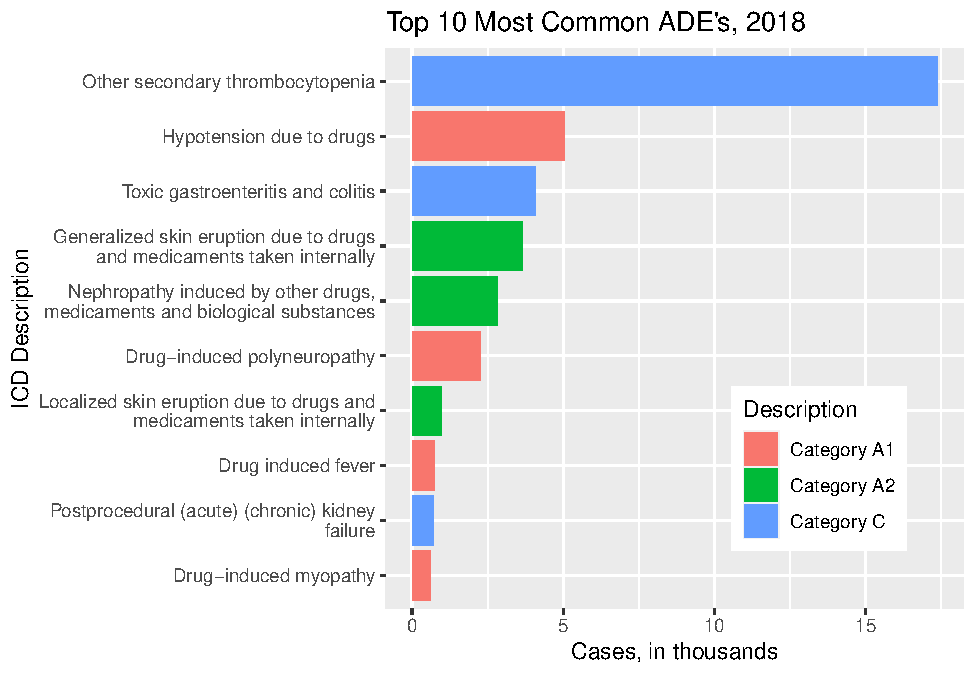
\includegraphics{final-project-paper_files/figure-latex/top-10-ade-1.pdf}

\begin{Shaded}
\begin{Highlighting}[]
\NormalTok{ade\_counts2 \textless{}{-}}\StringTok{ }\NormalTok{ade\_flag }\OperatorTok{\%\textgreater{}\%}
\StringTok{  }\KeywordTok{filter}\NormalTok{(has\_ade }\OperatorTok{==}\StringTok{ }\DecValTok{1}\NormalTok{) }\OperatorTok{\%\textgreater{}\%}
\StringTok{  }\KeywordTok{filter}\NormalTok{(Description }\OperatorTok{!=}\StringTok{ \textquotesingle{}Category C\textquotesingle{}}\NormalTok{) }\OperatorTok{\%\textgreater{}\%}
\StringTok{  }\KeywordTok{group\_by}\NormalTok{(Code, Description) }\OperatorTok{\%\textgreater{}\%}
\StringTok{  }\KeywordTok{summarize}\NormalTok{(}\DataTypeTok{n\_icd =} \KeywordTok{n}\NormalTok{()) }\OperatorTok{\%\textgreater{}\%}
\StringTok{  }\KeywordTok{left\_join}\NormalTok{(icd, }\KeywordTok{c}\NormalTok{(}\StringTok{\textquotesingle{}Code\textquotesingle{}}\NormalTok{ =}\StringTok{ \textquotesingle{}V3\textquotesingle{}}\NormalTok{)) }\OperatorTok{\%\textgreater{}\%}
\StringTok{  }\KeywordTok{arrange}\NormalTok{(}\KeywordTok{desc}\NormalTok{(n\_icd)) }\OperatorTok{\%\textgreater{}\%}
\StringTok{  }\KeywordTok{mutate}\NormalTok{(}\DataTypeTok{Description =} \KeywordTok{fct\_relevel}\NormalTok{(Description, }\KeywordTok{c}\NormalTok{(}\StringTok{\textquotesingle{}Category A1\textquotesingle{}}\NormalTok{,}\StringTok{\textquotesingle{}Category A2\textquotesingle{}}\NormalTok{, }\StringTok{\textquotesingle{}Category B2\textquotesingle{}}\NormalTok{, }\StringTok{\textquotesingle{}Category C\textquotesingle{}}\NormalTok{)))}
\end{Highlighting}
\end{Shaded}

\begin{verbatim}
## `summarise()` has grouped output by 'Code'. You can override using the
## `.groups` argument.
\end{verbatim}

\begin{verbatim}
## Warning: Unknown levels in `f`: Category A2, Category B2, Category C

## Warning: Unknown levels in `f`: Category A2, Category B2, Category C

## Warning: Unknown levels in `f`: Category A2, Category B2, Category C
\end{verbatim}

\begin{verbatim}
## Warning: Unknown levels in `f`: Category A1, Category B2, Category C

## Warning: Unknown levels in `f`: Category A1, Category B2, Category C
\end{verbatim}

\begin{verbatim}
## Warning: Unknown levels in `f`: Category A2, Category B2, Category C

## Warning: Unknown levels in `f`: Category A2, Category B2, Category C

## Warning: Unknown levels in `f`: Category A2, Category B2, Category C

## Warning: Unknown levels in `f`: Category A2, Category B2, Category C

## Warning: Unknown levels in `f`: Category A2, Category B2, Category C
\end{verbatim}

\begin{verbatim}
## Warning: Unknown levels in `f`: Category A1, Category A2, Category C

## Warning: Unknown levels in `f`: Category A1, Category A2, Category C

## Warning: Unknown levels in `f`: Category A1, Category A2, Category C

## Warning: Unknown levels in `f`: Category A1, Category A2, Category C
\end{verbatim}

\begin{verbatim}
## Warning: Unknown levels in `f`: Category A2, Category B2, Category C
\end{verbatim}

\begin{verbatim}
## Warning: Unknown levels in `f`: Category A1, Category B2, Category C
\end{verbatim}

\begin{verbatim}
## Warning: Unknown levels in `f`: Category A2, Category B2, Category C

## Warning: Unknown levels in `f`: Category A2, Category B2, Category C

## Warning: Unknown levels in `f`: Category A2, Category B2, Category C

## Warning: Unknown levels in `f`: Category A2, Category B2, Category C
\end{verbatim}

\begin{verbatim}
## Warning: Unknown levels in `f`: Category A1, Category B2, Category C
\end{verbatim}

\begin{verbatim}
## Warning: Unknown levels in `f`: Category A2, Category B2, Category C

## Warning: Unknown levels in `f`: Category A2, Category B2, Category C

## Warning: Unknown levels in `f`: Category A2, Category B2, Category C

## Warning: Unknown levels in `f`: Category A2, Category B2, Category C

## Warning: Unknown levels in `f`: Category A2, Category B2, Category C

## Warning: Unknown levels in `f`: Category A2, Category B2, Category C

## Warning: Unknown levels in `f`: Category A2, Category B2, Category C
\end{verbatim}

\begin{verbatim}
## Warning: Unknown levels in `f`: Category A1, Category B2, Category C

## Warning: Unknown levels in `f`: Category A1, Category B2, Category C

## Warning: Unknown levels in `f`: Category A1, Category B2, Category C

## Warning: Unknown levels in `f`: Category A1, Category B2, Category C

## Warning: Unknown levels in `f`: Category A1, Category B2, Category C

## Warning: Unknown levels in `f`: Category A1, Category B2, Category C

## Warning: Unknown levels in `f`: Category A1, Category B2, Category C
\end{verbatim}

\begin{verbatim}
## Warning: Unknown levels in `f`: Category A2, Category B2, Category C

## Warning: Unknown levels in `f`: Category A2, Category B2, Category C

## Warning: Unknown levels in `f`: Category A2, Category B2, Category C

## Warning: Unknown levels in `f`: Category A2, Category B2, Category C

## Warning: Unknown levels in `f`: Category A2, Category B2, Category C
\end{verbatim}

\begin{verbatim}
## Warning: Unknown levels in `f`: Category A1, Category B2, Category C
\end{verbatim}

\begin{verbatim}
## Warning: Unknown levels in `f`: Category A2, Category B2, Category C

## Warning: Unknown levels in `f`: Category A2, Category B2, Category C

## Warning: Unknown levels in `f`: Category A2, Category B2, Category C
\end{verbatim}

\begin{verbatim}
## Warning: Unknown levels in `f`: Category A1, Category B2, Category C

## Warning: Unknown levels in `f`: Category A1, Category B2, Category C

## Warning: Unknown levels in `f`: Category A1, Category B2, Category C

## Warning: Unknown levels in `f`: Category A1, Category B2, Category C
\end{verbatim}

\begin{verbatim}
## Warning: Unknown levels in `f`: Category A2, Category B2, Category C

## Warning: Unknown levels in `f`: Category A2, Category B2, Category C

## Warning: Unknown levels in `f`: Category A2, Category B2, Category C
\end{verbatim}

\begin{Shaded}
\begin{Highlighting}[]
\NormalTok{ade\_counts2 }\OperatorTok{\%\textgreater{}\%}
\StringTok{  }\KeywordTok{head}\NormalTok{(}\DecValTok{10}\NormalTok{) }\OperatorTok{\%\textgreater{}\%}
\StringTok{  }\KeywordTok{ggplot}\NormalTok{(}\KeywordTok{aes}\NormalTok{(}\DataTypeTok{x =} \KeywordTok{fct\_reorder}\NormalTok{(V5, n\_icd))) }\OperatorTok{+}
\StringTok{  }\KeywordTok{geom\_col}\NormalTok{(}\KeywordTok{aes}\NormalTok{(}\DataTypeTok{y =}\NormalTok{ n\_icd}\OperatorTok{/}\DecValTok{1000}\NormalTok{, }\DataTypeTok{fill =}\NormalTok{ Description)) }\OperatorTok{+}\StringTok{ }
\StringTok{  }\KeywordTok{scale\_x\_discrete}\NormalTok{(}\DataTypeTok{name =} \StringTok{\textquotesingle{}ICD Description\textquotesingle{}}\NormalTok{, }\DataTypeTok{labels =} \ControlFlowTok{function}\NormalTok{(x) }\KeywordTok{str\_wrap}\NormalTok{(}\KeywordTok{str\_replace\_all}\NormalTok{(x, }\StringTok{"foo"}\NormalTok{ , }\StringTok{" "}\NormalTok{),}
                                                 \DataTypeTok{width =} \DecValTok{40}\NormalTok{)) }\OperatorTok{+}
\StringTok{  }\KeywordTok{theme}\NormalTok{(}\DataTypeTok{legend.position =} \KeywordTok{c}\NormalTok{(}\FloatTok{0.75}\NormalTok{,}\FloatTok{0.25}\NormalTok{)) }\OperatorTok{+}
\StringTok{  }\KeywordTok{labs}\NormalTok{(}\DataTypeTok{title =} \StringTok{\textquotesingle{}Most Common Category }\CharTok{\textbackslash{}\textquotesingle{}}\StringTok{A}\CharTok{\textbackslash{}\textquotesingle{}}\StringTok{ drug reactions\textquotesingle{}}\NormalTok{) }\OperatorTok{+}
\StringTok{  }\KeywordTok{scale\_y\_continuous}\NormalTok{(}\DataTypeTok{name =} \StringTok{\textquotesingle{}Cases, in thousands\textquotesingle{}}\NormalTok{) }\OperatorTok{+}
\StringTok{  }\KeywordTok{coord\_flip}\NormalTok{() }
\end{Highlighting}
\end{Shaded}

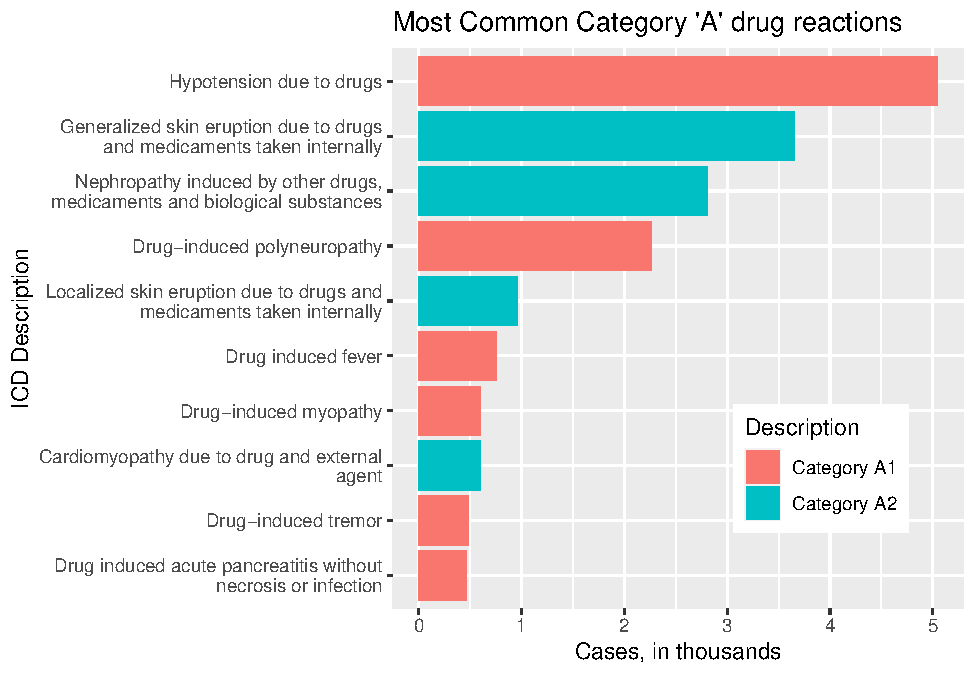
\includegraphics{final-project-paper_files/figure-latex/top-10-ade-cat-ab-1.pdf}

\begin{Shaded}
\begin{Highlighting}[]
\NormalTok{ade\_counts2 }\OperatorTok{\%\textgreater{}\%}
\StringTok{  }\KeywordTok{filter}\NormalTok{(Description }\OperatorTok{==}\StringTok{ \textquotesingle{}Category B2\textquotesingle{}}\NormalTok{) }\OperatorTok{\%\textgreater{}\%}
\StringTok{  }\KeywordTok{head}\NormalTok{(}\DecValTok{10}\NormalTok{) }\OperatorTok{\%\textgreater{}\%}
\StringTok{  }\KeywordTok{ggplot}\NormalTok{(}\KeywordTok{aes}\NormalTok{(}\DataTypeTok{x =} \KeywordTok{fct\_reorder}\NormalTok{(V5, n\_icd))) }\OperatorTok{+}
\StringTok{  }\KeywordTok{geom\_col}\NormalTok{(}\KeywordTok{aes}\NormalTok{(}\DataTypeTok{y =}\NormalTok{ n\_icd)) }\OperatorTok{+}\StringTok{ }
\StringTok{  }\KeywordTok{scale\_x\_discrete}\NormalTok{(}\DataTypeTok{name =} \StringTok{\textquotesingle{}ICD Description\textquotesingle{}}\NormalTok{, }\DataTypeTok{labels =} \ControlFlowTok{function}\NormalTok{(x) }\KeywordTok{str\_wrap}\NormalTok{(}\KeywordTok{str\_replace\_all}\NormalTok{(x, }\StringTok{"foo"}\NormalTok{ , }\StringTok{" "}\NormalTok{),}
                                                 \DataTypeTok{width =} \DecValTok{35}\NormalTok{)) }\OperatorTok{+}
\StringTok{  }\KeywordTok{labs}\NormalTok{(}\DataTypeTok{title =} \StringTok{\textquotesingle{}Most Common Category }\CharTok{\textbackslash{}\textquotesingle{}}\StringTok{B}\CharTok{\textbackslash{}\textquotesingle{}}\StringTok{ drug reactions\textquotesingle{}}\NormalTok{) }\OperatorTok{+}
\StringTok{  }\KeywordTok{scale\_y\_continuous}\NormalTok{(}\DataTypeTok{name =} \StringTok{\textquotesingle{}Cases\textquotesingle{}}\NormalTok{) }\OperatorTok{+}
\StringTok{  }\KeywordTok{coord\_flip}\NormalTok{() }
\end{Highlighting}
\end{Shaded}

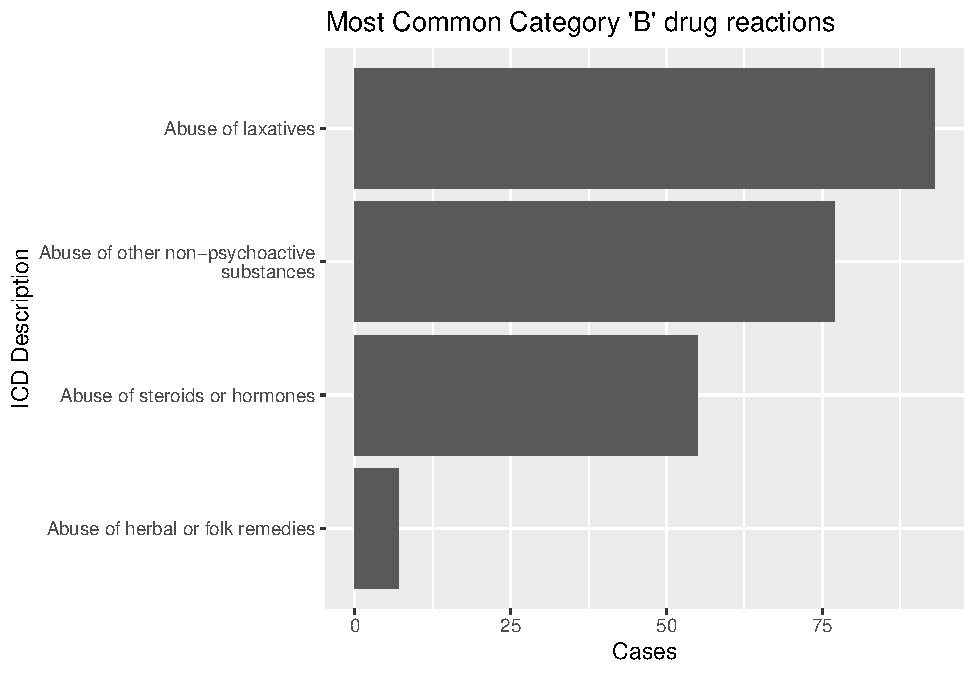
\includegraphics{final-project-paper_files/figure-latex/top-10-ade-cat-ab-2.pdf}

\begin{Shaded}
\begin{Highlighting}[]
\NormalTok{ade\_counts }\OperatorTok{\%\textgreater{}\%}
\StringTok{  }\KeywordTok{filter}\NormalTok{(Description }\OperatorTok{==}\StringTok{ \textquotesingle{}Category C\textquotesingle{}}\NormalTok{) }\OperatorTok{\%\textgreater{}\%}
\StringTok{  }\KeywordTok{head}\NormalTok{(}\DecValTok{3}\NormalTok{) }\OperatorTok{\%\textgreater{}\%}
\StringTok{  }\KeywordTok{ggplot}\NormalTok{(}\KeywordTok{aes}\NormalTok{(}\DataTypeTok{x =} \KeywordTok{fct\_reorder}\NormalTok{(V5, n\_icd))) }\OperatorTok{+}
\StringTok{  }\KeywordTok{geom\_col}\NormalTok{(}\KeywordTok{aes}\NormalTok{(}\DataTypeTok{y =}\NormalTok{ n\_icd}\OperatorTok{/}\DecValTok{1000}\NormalTok{)) }\OperatorTok{+}\StringTok{ }
\StringTok{  }\KeywordTok{scale\_x\_discrete}\NormalTok{(}\DataTypeTok{name =} \StringTok{\textquotesingle{}ICD Description\textquotesingle{}}\NormalTok{, }\DataTypeTok{labels =} \ControlFlowTok{function}\NormalTok{(x) }\KeywordTok{str\_wrap}\NormalTok{(}\KeywordTok{str\_replace\_all}\NormalTok{(x, }\StringTok{"foo"}\NormalTok{ , }\StringTok{" "}\NormalTok{),}
                                                 \DataTypeTok{width =} \DecValTok{35}\NormalTok{)) }\OperatorTok{+}
\StringTok{  }\KeywordTok{labs}\NormalTok{(}\DataTypeTok{title =} \StringTok{\textquotesingle{}Most Common Category }\CharTok{\textbackslash{}\textquotesingle{}}\StringTok{C}\CharTok{\textbackslash{}\textquotesingle{}}\StringTok{ drug reactions\textquotesingle{}}\NormalTok{) }\OperatorTok{+}
\StringTok{  }\KeywordTok{scale\_y\_continuous}\NormalTok{(}\DataTypeTok{name =} \StringTok{\textquotesingle{}Cases, in thousands\textquotesingle{}}\NormalTok{) }\OperatorTok{+}
\StringTok{  }\KeywordTok{coord\_flip}\NormalTok{() }
\end{Highlighting}
\end{Shaded}

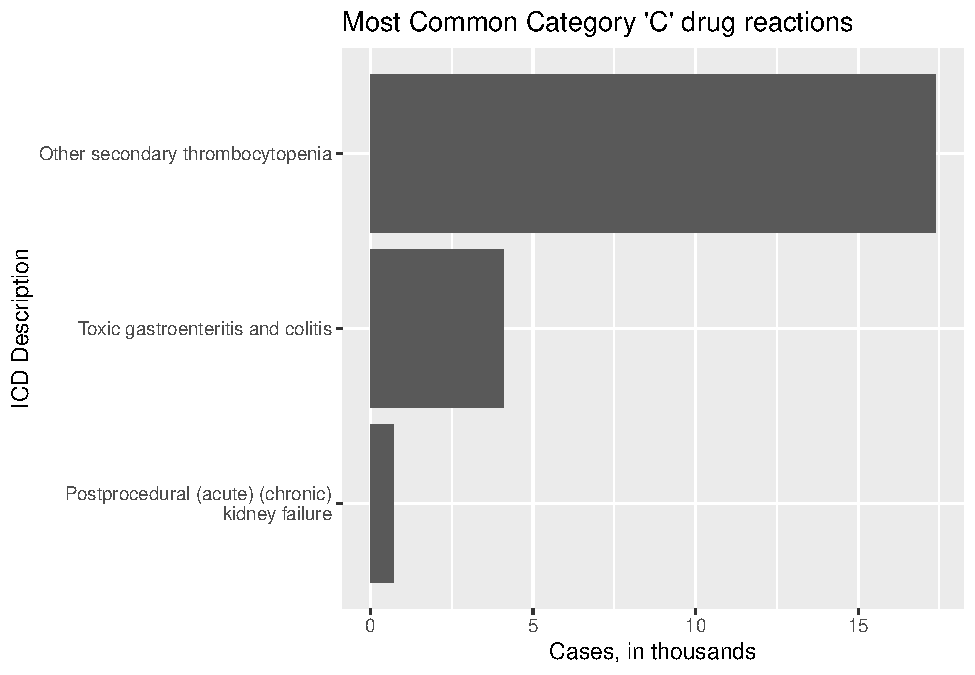
\includegraphics{final-project-paper_files/figure-latex/top-10-ade-cat-ab-3.pdf}

\begin{Shaded}
\begin{Highlighting}[]
\KeywordTok{ggplot}\NormalTok{(ade\_flag, }\KeywordTok{aes}\NormalTok{(I10\_NDX)) }\OperatorTok{+}\StringTok{ }\CommentTok{\#anomaly in the number of diagnoses}
\StringTok{  }\KeywordTok{geom\_bar}\NormalTok{() }\OperatorTok{+}
\StringTok{  }\KeywordTok{geom\_vline}\NormalTok{(}\DataTypeTok{xintercept =} \DecValTok{25}\NormalTok{) }\OperatorTok{+}
\StringTok{  }\KeywordTok{labs}\NormalTok{(}\DataTypeTok{x =} \StringTok{\textquotesingle{}Number of ICD Diagnoses per Patient\textquotesingle{}}\NormalTok{, }\DataTypeTok{y =} \StringTok{\textquotesingle{}Count\textquotesingle{}}\NormalTok{, }\DataTypeTok{title =} \StringTok{\textquotesingle{}Unexpected Mode for ICD Diagnoses\textquotesingle{}}\NormalTok{)}
\end{Highlighting}
\end{Shaded}

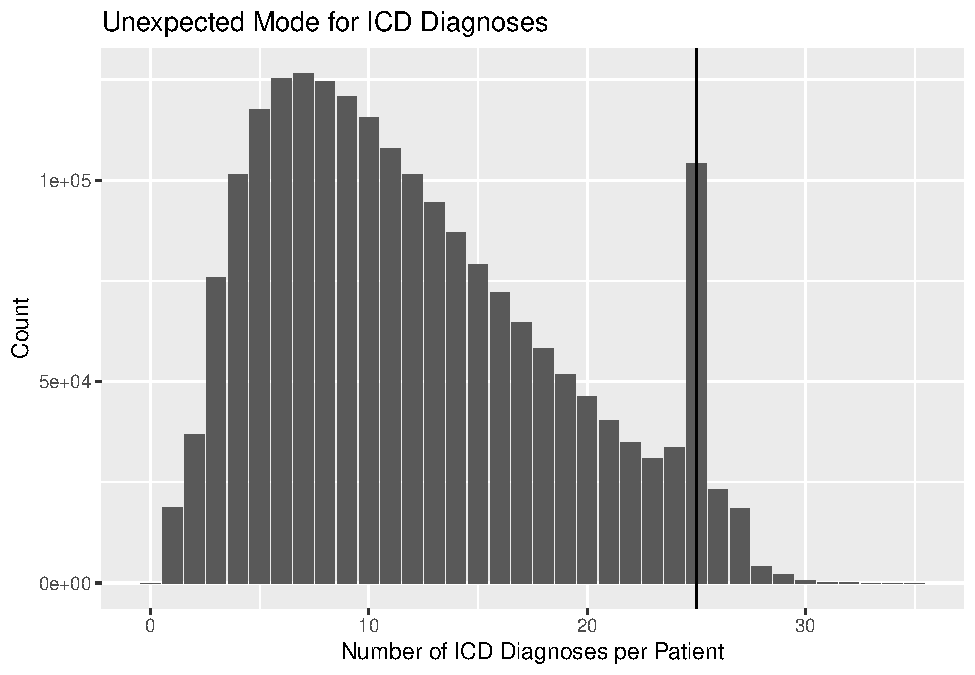
\includegraphics{final-project-paper_files/figure-latex/n-Diagnoses-1.pdf}

\begin{Shaded}
\begin{Highlighting}[]
\NormalTok{i10\_procedure \textless{}{-}}\StringTok{ }\KeywordTok{read.csv}\NormalTok{(}\StringTok{"i10\_procedure.csv"}\NormalTok{, }\DataTypeTok{stringsAsFactors =} \OtherTok{TRUE}\NormalTok{) }\CommentTok{\#icd 10 procedure codes}

\NormalTok{charge\_codes \textless{}{-}}\StringTok{ }\KeywordTok{read.csv}\NormalTok{(}\StringTok{\textquotesingle{}revcodes.csv\textquotesingle{}}\NormalTok{)}

\CommentTok{\#NY\_FIPS \textless{}{-} read.csv(\textquotesingle{}NY\_Municipalities\_and\_County\_FIPS\_codes.csv\textquotesingle{})}
\CommentTok{\#NY\_FIPS$County.FIPS[NY\_FIPS$County.Name == \textquotesingle{}St Lawrence\textquotesingle{}] \textless{}{-} 36089}
\CommentTok{\#NY\_FIPS$County.FIPS \textless{}{-} as.factor(NY\_FIPS$County.FIPS)}
\end{Highlighting}
\end{Shaded}

\begin{Shaded}
\begin{Highlighting}[]
\NormalTok{icd \textless{}{-}}\StringTok{ }\NormalTok{icd }\OperatorTok{\%\textgreater{}\%}\StringTok{ }\CommentTok{\#recoded icd csv with icd dx categories}
\StringTok{  }\KeywordTok{mutate}\NormalTok{(}\DataTypeTok{icd\_cat =} \KeywordTok{case\_when}\NormalTok{(}\KeywordTok{substr}\NormalTok{(V1,}\DecValTok{1}\NormalTok{,}\DecValTok{1}\NormalTok{) }\OperatorTok{==}\StringTok{ "A"} \OperatorTok{|}\StringTok{ }\KeywordTok{substr}\NormalTok{(V1,}\DecValTok{1}\NormalTok{,}\DecValTok{1}\NormalTok{) }\OperatorTok{==}\StringTok{ "B"} \OperatorTok{\textasciitilde{}}\StringTok{ \textquotesingle{}Certain infections and parasitic diseases\textquotesingle{}}\NormalTok{,}
                             \KeywordTok{substr}\NormalTok{(V1,}\DecValTok{1}\NormalTok{,}\DecValTok{1}\NormalTok{) }\OperatorTok{==}\StringTok{ "C"} \OperatorTok{\textasciitilde{}}\StringTok{ \textquotesingle{}Neoplasms\textquotesingle{}}\NormalTok{,}
                             \KeywordTok{substr}\NormalTok{(V1,}\DecValTok{1}\NormalTok{,}\DecValTok{1}\NormalTok{) }\OperatorTok{==}\StringTok{ "D"} \OperatorTok{\textasciitilde{}}\StringTok{ \textquotesingle{}Diseases of the blood and blood{-}forming organ\textquotesingle{}}\NormalTok{,}
                              \KeywordTok{substr}\NormalTok{(V1,}\DecValTok{1}\NormalTok{,}\DecValTok{1}\NormalTok{) }\OperatorTok{==}\StringTok{ "E"} \OperatorTok{\textasciitilde{}}\StringTok{ \textquotesingle{}Endocrine, nutritional and metabolic diseases\textquotesingle{}}\NormalTok{,}
                              \KeywordTok{substr}\NormalTok{(V1,}\DecValTok{1}\NormalTok{,}\DecValTok{1}\NormalTok{) }\OperatorTok{==}\StringTok{ "F"} \OperatorTok{\textasciitilde{}}\StringTok{ \textquotesingle{}Mental, Behavioral and Neurodevelopmental disorders\textquotesingle{}}\NormalTok{,}
                              \KeywordTok{substr}\NormalTok{(V1,}\DecValTok{1}\NormalTok{,}\DecValTok{1}\NormalTok{) }\OperatorTok{==}\StringTok{ "G"} \OperatorTok{\textasciitilde{}}\StringTok{ \textquotesingle{}Diseases of the nervous system\textquotesingle{}}\NormalTok{,}
                              \KeywordTok{substr}\NormalTok{(V1,}\DecValTok{1}\NormalTok{,}\DecValTok{1}\NormalTok{) }\OperatorTok{==}\StringTok{ "H"} \OperatorTok{\&}\StringTok{ }\KeywordTok{as.numeric}\NormalTok{(}\KeywordTok{substr}\NormalTok{(V1, }\DecValTok{2}\NormalTok{,}\DecValTok{2}\NormalTok{)) }\OperatorTok{\textless{}=}\DecValTok{5} \OperatorTok{\textasciitilde{}}\StringTok{ \textquotesingle{}Diseases of the eye and adnexa\textquotesingle{}}\NormalTok{,}
                              \KeywordTok{substr}\NormalTok{(V1,}\DecValTok{1}\NormalTok{,}\DecValTok{1}\NormalTok{) }\OperatorTok{==}\StringTok{ "H"} \OperatorTok{\&}\StringTok{ }\KeywordTok{as.numeric}\NormalTok{(}\KeywordTok{substr}\NormalTok{(V1, }\DecValTok{2}\NormalTok{,}\DecValTok{2}\NormalTok{)) }\OperatorTok{\textgreater{}}\DecValTok{5} \OperatorTok{\textasciitilde{}}\StringTok{ \textquotesingle{}    Diseases of the ear and mastoid process\textquotesingle{}}\NormalTok{,}
                              \KeywordTok{substr}\NormalTok{(V1,}\DecValTok{1}\NormalTok{,}\DecValTok{1}\NormalTok{) }\OperatorTok{==}\StringTok{ "I"} \OperatorTok{\textasciitilde{}}\StringTok{ \textquotesingle{}Diseases of the circulatory system\textquotesingle{}}\NormalTok{,}
                              \KeywordTok{substr}\NormalTok{(V1,}\DecValTok{1}\NormalTok{,}\DecValTok{1}\NormalTok{) }\OperatorTok{==}\StringTok{ "J"} \OperatorTok{\textasciitilde{}}\StringTok{ \textquotesingle{}Diseases of the respiratory system\textquotesingle{}}\NormalTok{,}
                              \KeywordTok{substr}\NormalTok{(V1,}\DecValTok{1}\NormalTok{,}\DecValTok{1}\NormalTok{) }\OperatorTok{==}\StringTok{ "K"} \OperatorTok{\textasciitilde{}}\StringTok{ \textquotesingle{}Diseases of the digestive system\textquotesingle{}}\NormalTok{,}
                              \KeywordTok{substr}\NormalTok{(V1,}\DecValTok{1}\NormalTok{,}\DecValTok{1}\NormalTok{) }\OperatorTok{==}\StringTok{ "L"} \OperatorTok{\textasciitilde{}}\StringTok{ \textquotesingle{}Diseases of the skin and subcutaneous tissue\textquotesingle{}}\NormalTok{,}
                              \KeywordTok{substr}\NormalTok{(V1,}\DecValTok{1}\NormalTok{,}\DecValTok{1}\NormalTok{) }\OperatorTok{==}\StringTok{ "M"} \OperatorTok{\textasciitilde{}}\StringTok{ \textquotesingle{}Diseases of the musculoskeletal system and connective tissue\textquotesingle{}}\NormalTok{,}
                              \KeywordTok{substr}\NormalTok{(V1,}\DecValTok{1}\NormalTok{,}\DecValTok{1}\NormalTok{) }\OperatorTok{==}\StringTok{ "N"} \OperatorTok{\textasciitilde{}}\StringTok{ \textquotesingle{}Diseases of the genitourinary system\textquotesingle{}}\NormalTok{,}
                              \KeywordTok{substr}\NormalTok{(V1,}\DecValTok{1}\NormalTok{,}\DecValTok{1}\NormalTok{) }\OperatorTok{==}\StringTok{ "O"} \OperatorTok{\textasciitilde{}}\StringTok{ \textquotesingle{}Pregnancy, childbirth, and puerperium\textquotesingle{}}\NormalTok{,}
                              \KeywordTok{substr}\NormalTok{(V1,}\DecValTok{1}\NormalTok{,}\DecValTok{1}\NormalTok{) }\OperatorTok{==}\StringTok{ "P"} \OperatorTok{\textasciitilde{}}\StringTok{ \textquotesingle{}Certain conditions originating in the perinatal period\textquotesingle{}}\NormalTok{,}
                              \KeywordTok{substr}\NormalTok{(V1,}\DecValTok{1}\NormalTok{,}\DecValTok{1}\NormalTok{) }\OperatorTok{==}\StringTok{ "Q"} \OperatorTok{\textasciitilde{}}\StringTok{ \textquotesingle{}Congenital malformations, deformations and chromosomal abnormalities\textquotesingle{}}\NormalTok{,}
                              \KeywordTok{substr}\NormalTok{(V1,}\DecValTok{1}\NormalTok{,}\DecValTok{1}\NormalTok{) }\OperatorTok{==}\StringTok{ "R"} \OperatorTok{\textasciitilde{}}\StringTok{ \textquotesingle{}Symptoms, signs, and abnormal clinical laboratory findings, not elsewhere classified\textquotesingle{}}\NormalTok{,}
                              \KeywordTok{substr}\NormalTok{(V1,}\DecValTok{1}\NormalTok{,}\DecValTok{1}\NormalTok{) }\OperatorTok{==}\StringTok{ "S"} \OperatorTok{|}\StringTok{ }\KeywordTok{substr}\NormalTok{(V1,}\DecValTok{1}\NormalTok{,}\DecValTok{1}\NormalTok{) }\OperatorTok{==}\StringTok{ "T"} \OperatorTok{\textasciitilde{}}\StringTok{ \textquotesingle{}Injury, poisoning, and certain other consequences of external causes\textquotesingle{}}\NormalTok{,}
                              \KeywordTok{substr}\NormalTok{(V1,}\DecValTok{1}\NormalTok{,}\DecValTok{1}\NormalTok{) }\OperatorTok{==}\StringTok{ "V"} \OperatorTok{|}\StringTok{ }\KeywordTok{substr}\NormalTok{(V1,}\DecValTok{1}\NormalTok{,}\DecValTok{1}\NormalTok{) }\OperatorTok{==}\StringTok{ "W"} \OperatorTok{|}\StringTok{ }\KeywordTok{substr}\NormalTok{(V1,}\DecValTok{1}\NormalTok{,}\DecValTok{1}\NormalTok{) }\OperatorTok{==}\StringTok{ "X"} \OperatorTok{|}\StringTok{ }\KeywordTok{substr}\NormalTok{(V1,}\DecValTok{1}\NormalTok{,}\DecValTok{1}\NormalTok{) }\OperatorTok{==}\StringTok{ "Y"} \OperatorTok{\textasciitilde{}}\StringTok{ \textquotesingle{}External causes of morbidity\textquotesingle{}}\NormalTok{,}
                              \KeywordTok{substr}\NormalTok{(V1,}\DecValTok{1}\NormalTok{,}\DecValTok{1}\NormalTok{) }\OperatorTok{==}\StringTok{ "Z"} \OperatorTok{\textasciitilde{}}\StringTok{ \textquotesingle{}Factors influencing health status and contact with health services\textquotesingle{}}
\NormalTok{                             )}
\NormalTok{         )}
\end{Highlighting}
\end{Shaded}

\begin{Shaded}
\begin{Highlighting}[]
\CommentTok{\#\#\#{-}Proportion of women (+ SD) }
\NormalTok{ade\_flag }\OperatorTok{\%\textgreater{}\%}
\StringTok{    }\KeywordTok{summarize}\NormalTok{(}\DataTypeTok{avg\_female =} \KeywordTok{mean}\NormalTok{((FEMALE }\OperatorTok{==}\StringTok{ }\DecValTok{1}\NormalTok{), }\DataTypeTok{na.rm =} \OtherTok{TRUE}\NormalTok{))}
\end{Highlighting}
\end{Shaded}

\begin{verbatim}
## # A tibble: 1 x 1
##   avg_female
##        <dbl>
## 1      0.562
\end{verbatim}

\begin{Shaded}
\begin{Highlighting}[]
\NormalTok{ade\_flag }\OperatorTok{\%\textgreater{}\%}
\StringTok{    }\KeywordTok{summarize}\NormalTok{(}\DataTypeTok{sd\_female =} \KeywordTok{sd}\NormalTok{(}\KeywordTok{as.numeric}\NormalTok{(FEMALE }\OperatorTok{==}\StringTok{ }\DecValTok{1}\NormalTok{), }\DataTypeTok{na.rm =} \OtherTok{TRUE}\NormalTok{))}
\end{Highlighting}
\end{Shaded}

\begin{verbatim}
## # A tibble: 1 x 1
##   sd_female
##       <dbl>
## 1     0.496
\end{verbatim}

\begin{Shaded}
\begin{Highlighting}[]
\CommentTok{\#\#{-}Proportion of races }
\NormalTok{ade\_flag }\OperatorTok{\%\textgreater{}\%}
\StringTok{    }\KeywordTok{mutate}\NormalTok{(}\DataTypeTok{RACE =} \KeywordTok{recode\_factor}\NormalTok{(RACE, }\StringTok{\textasciigrave{}}\DataTypeTok{1}\StringTok{\textasciigrave{}}\NormalTok{=}\StringTok{ \textquotesingle{}White\textquotesingle{}}\NormalTok{,}
                                                            \StringTok{\textasciigrave{}}\DataTypeTok{2}\StringTok{\textasciigrave{}}\NormalTok{ =}\StringTok{ \textquotesingle{}Black\textquotesingle{}}\NormalTok{,}
                                                            \StringTok{\textasciigrave{}}\DataTypeTok{3}\StringTok{\textasciigrave{}}\NormalTok{ =}\StringTok{ \textquotesingle{}Hispanic\textquotesingle{}}\NormalTok{,}
                                                            \StringTok{\textasciigrave{}}\DataTypeTok{4}\StringTok{\textasciigrave{}}\NormalTok{ =}\StringTok{ \textquotesingle{}AAPI\textquotesingle{}}\NormalTok{,}
                                                            \StringTok{\textasciigrave{}}\DataTypeTok{5}\StringTok{\textasciigrave{}}\NormalTok{ =}\StringTok{ \textquotesingle{}Native American\textquotesingle{}}\NormalTok{,}
                                                            \StringTok{\textasciigrave{}}\DataTypeTok{6}\StringTok{\textasciigrave{}}\NormalTok{ =}\StringTok{ \textquotesingle{}Other/Missing\textquotesingle{}}\NormalTok{,}
                                                            \StringTok{\textasciigrave{}}\DataTypeTok{NA}\StringTok{\textasciigrave{}}\NormalTok{ =}\StringTok{ \textquotesingle{}Other/Missing\textquotesingle{}}\NormalTok{)) }\OperatorTok{\%\textgreater{}\%}
\StringTok{    }\KeywordTok{group\_by}\NormalTok{(RACE) }\OperatorTok{\%\textgreater{}\%}
\StringTok{    }\KeywordTok{summarize}\NormalTok{(}\DataTypeTok{PCT\_RACE =} \DecValTok{100}\OperatorTok{*}\KeywordTok{round}\NormalTok{(}\KeywordTok{n}\NormalTok{()}\OperatorTok{/}\KeywordTok{nrow}\NormalTok{(ade\_flag),}\DecValTok{3}\NormalTok{))}
\end{Highlighting}
\end{Shaded}

\begin{verbatim}
## Warning in recode.numeric(.x, !!!values, .default = .default, .missing
## = .missing): NAs introduced by coercion
\end{verbatim}

\begin{verbatim}
## # A tibble: 6 x 2
##   RACE            PCT_RACE
##   <fct>              <dbl>
## 1 White               54.6
## 2 Black               17.1
## 3 Hispanic            13.8
## 4 AAPI                 4.6
## 5 Native American      0.2
## 6 Other/Missing        9.7
\end{verbatim}

\begin{Shaded}
\begin{Highlighting}[]
\CommentTok{\#\#{-}Proportion Hispanic }

\NormalTok{ade\_flag }\OperatorTok{\%\textgreater{}\%}
\StringTok{  }\KeywordTok{mutate}\NormalTok{(}\DataTypeTok{HISPANIC =} \KeywordTok{na\_if}\NormalTok{(HISPANIC, }\StringTok{\textquotesingle{}\textquotesingle{}}\NormalTok{)) }\OperatorTok{\%\textgreater{}\%}
\StringTok{    }\KeywordTok{mutate}\NormalTok{(}\DataTypeTok{HISPANIC =} \KeywordTok{recode\_factor}\NormalTok{(HISPANIC, }\StringTok{\textasciigrave{}}\DataTypeTok{0}\StringTok{\textasciigrave{}}\NormalTok{=}\StringTok{ \textquotesingle{}Not Hispanic\textquotesingle{}}\NormalTok{,}
                                                            \StringTok{\textasciigrave{}}\DataTypeTok{1}\StringTok{\textasciigrave{}}\NormalTok{ =}\StringTok{ \textquotesingle{}Hispanic, White\textquotesingle{}}\NormalTok{,}
                                                            \StringTok{\textasciigrave{}}\DataTypeTok{2}\StringTok{\textasciigrave{}}\NormalTok{ =}\StringTok{ \textquotesingle{}Hispanic, Black\textquotesingle{}}\NormalTok{,}
                                                            \StringTok{\textasciigrave{}}\DataTypeTok{3}\StringTok{\textasciigrave{}}\NormalTok{ =}\StringTok{ \textquotesingle{}Hispanic, Other Race\textquotesingle{}}\NormalTok{)) }\OperatorTok{\%\textgreater{}\%}
\StringTok{    }\KeywordTok{group\_by}\NormalTok{(HISPANIC) }\OperatorTok{\%\textgreater{}\%}
\StringTok{    }\KeywordTok{summarize}\NormalTok{(}\DataTypeTok{PCT\_HISPANIC =} \DecValTok{100}\OperatorTok{*}\KeywordTok{round}\NormalTok{(}\KeywordTok{n}\NormalTok{()}\OperatorTok{/}\KeywordTok{nrow}\NormalTok{(ade\_flag),}\DecValTok{3}\NormalTok{))}
\end{Highlighting}
\end{Shaded}

\begin{verbatim}
## # A tibble: 5 x 2
##   HISPANIC             PCT_HISPANIC
##   <fct>                       <dbl>
## 1 Not Hispanic                 81.6
## 2 Hispanic, White               3.2
## 3 Hispanic, Black               0.7
## 4 Hispanic, Other Race          9.8
## 5 <NA>                          4.6
\end{verbatim}

\begin{Shaded}
\begin{Highlighting}[]
\CommentTok{\#\#{-}Average charge  }
\NormalTok{ade\_flag }\OperatorTok{\%\textgreater{}\%}
\StringTok{    }\KeywordTok{summarize}\NormalTok{(}\DataTypeTok{avg\_charge =} \KeywordTok{mean}\NormalTok{(TOTCHG\_X, }\DataTypeTok{na.rm =} \OtherTok{TRUE}\NormalTok{))}
\end{Highlighting}
\end{Shaded}

\begin{verbatim}
## # A tibble: 1 x 1
##   avg_charge
##        <dbl>
## 1     56840.
\end{verbatim}

\begin{Shaded}
\begin{Highlighting}[]
\KeywordTok{ggplot}\NormalTok{(ade\_flag, }\KeywordTok{aes}\NormalTok{(}\DataTypeTok{x =}\NormalTok{ TOTCHG\_X)) }\OperatorTok{+}
\StringTok{  }\KeywordTok{geom\_histogram}\NormalTok{() }\OperatorTok{+}
\StringTok{  }\KeywordTok{scale\_x\_continuous}\NormalTok{(}\DataTypeTok{trans =} \StringTok{\textquotesingle{}log10\textquotesingle{}}\NormalTok{, }\DataTypeTok{labels =}\NormalTok{ scales}\OperatorTok{::}\KeywordTok{dollar\_format}\NormalTok{()) }\OperatorTok{+}
\StringTok{  }\KeywordTok{labs}\NormalTok{(}\DataTypeTok{x =} \StringTok{\textquotesingle{}Total Charges per Visit, log scale\textquotesingle{}}\NormalTok{, }\DataTypeTok{y =} \StringTok{\textquotesingle{}Count\textquotesingle{}}\NormalTok{, }\DataTypeTok{title =} \StringTok{\textquotesingle{}Distribution of Charges, Inpatient Stays\textquotesingle{}}\NormalTok{)}
\end{Highlighting}
\end{Shaded}

\begin{verbatim}
## `stat_bin()` using `bins = 30`. Pick better value with `binwidth`.
\end{verbatim}

\begin{verbatim}
## Warning: Removed 19 rows containing non-finite values (stat_bin).
\end{verbatim}

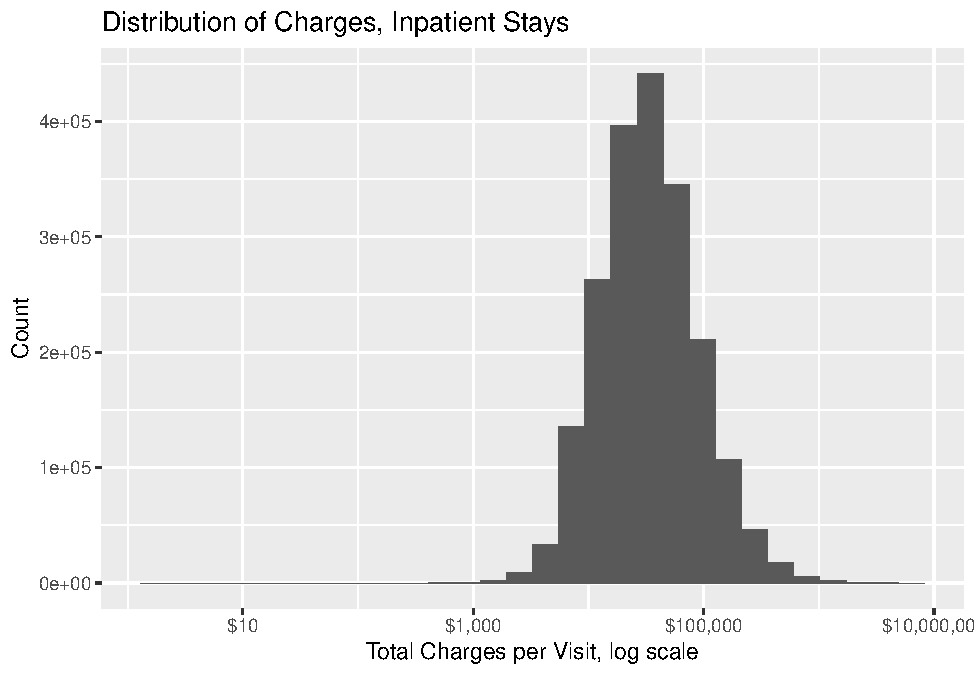
\includegraphics{final-project-paper_files/figure-latex/av-charge-1.pdf}

\begin{Shaded}
\begin{Highlighting}[]
\CommentTok{\#\#{-}Proportion of ED admissions }

\NormalTok{ade\_flag }\OperatorTok{\%\textgreater{}\%}
\StringTok{  }\KeywordTok{summarize}\NormalTok{(}\DataTypeTok{PCT\_ED =} \KeywordTok{mean}\NormalTok{(}\KeywordTok{as.numeric}\NormalTok{(HCUP\_ED }\OperatorTok{!=}\StringTok{ }\DecValTok{0}\NormalTok{)))}
\end{Highlighting}
\end{Shaded}

\begin{verbatim}
## # A tibble: 1 x 1
##   PCT_ED
##    <dbl>
## 1  0.670
\end{verbatim}

\begin{Shaded}
\begin{Highlighting}[]
\NormalTok{ade\_flag }\OperatorTok{\%\textgreater{}\%}
\StringTok{    }\KeywordTok{summarize}\NormalTok{(}\DataTypeTok{SD\_ED =} \KeywordTok{sd}\NormalTok{(}\KeywordTok{as.numeric}\NormalTok{(HCUP\_ED }\OperatorTok{!=}\StringTok{ }\DecValTok{0}\NormalTok{)))}
\end{Highlighting}
\end{Shaded}

\begin{verbatim}
## # A tibble: 1 x 1
##   SD_ED
##   <dbl>
## 1 0.470
\end{verbatim}

\begin{Shaded}
\begin{Highlighting}[]
\CommentTok{\#\#{-}Average LOS }

\NormalTok{ade\_flag }\OperatorTok{\%\textgreater{}\%}
\StringTok{    }\KeywordTok{summarize}\NormalTok{(}\DataTypeTok{AVG\_LOS =} \KeywordTok{mean}\NormalTok{(LOS\_X, }\DataTypeTok{na.rm =} \OtherTok{TRUE}\NormalTok{))}
\end{Highlighting}
\end{Shaded}

\begin{verbatim}
## # A tibble: 1 x 1
##   AVG_LOS
##     <dbl>
## 1    5.65
\end{verbatim}

\begin{Shaded}
\begin{Highlighting}[]
\NormalTok{ade\_flag }\OperatorTok{\%\textgreater{}\%}
\StringTok{  }\KeywordTok{summarize}\NormalTok{(}\DataTypeTok{SD\_LOS =} \KeywordTok{sd}\NormalTok{(LOS\_X, }\DataTypeTok{na.rm =} \OtherTok{TRUE}\NormalTok{))}
\end{Highlighting}
\end{Shaded}

\begin{verbatim}
## # A tibble: 1 x 1
##   SD_LOS
##    <dbl>
## 1   9.80
\end{verbatim}

\begin{Shaded}
\begin{Highlighting}[]
\KeywordTok{ggplot}\NormalTok{(ade\_flag, }\KeywordTok{aes}\NormalTok{(}\DataTypeTok{x =}\NormalTok{ LOS\_X)) }\OperatorTok{+}
\StringTok{  }\KeywordTok{geom\_histogram}\NormalTok{() }\OperatorTok{+}
\StringTok{  }\KeywordTok{scale\_x\_continuous}\NormalTok{(}\DataTypeTok{trans =} \StringTok{\textquotesingle{}log10\textquotesingle{}}\NormalTok{) }\OperatorTok{+}
\StringTok{  }\KeywordTok{labs}\NormalTok{(}\DataTypeTok{x =} \StringTok{\textquotesingle{}Total Length of Stay, log scale\textquotesingle{}}\NormalTok{, }\DataTypeTok{y =} \StringTok{\textquotesingle{}Count\textquotesingle{}}\NormalTok{, }\DataTypeTok{title =} \StringTok{\textquotesingle{}Length of Inpatient Stay\textquotesingle{}}\NormalTok{)}
\end{Highlighting}
\end{Shaded}

\begin{verbatim}
## Warning: Transformation introduced infinite values in continuous x-axis
\end{verbatim}

\begin{verbatim}
## `stat_bin()` using `bins = 30`. Pick better value with `binwidth`.
\end{verbatim}

\begin{verbatim}
## Warning: Removed 43456 rows containing non-finite values (stat_bin).
\end{verbatim}

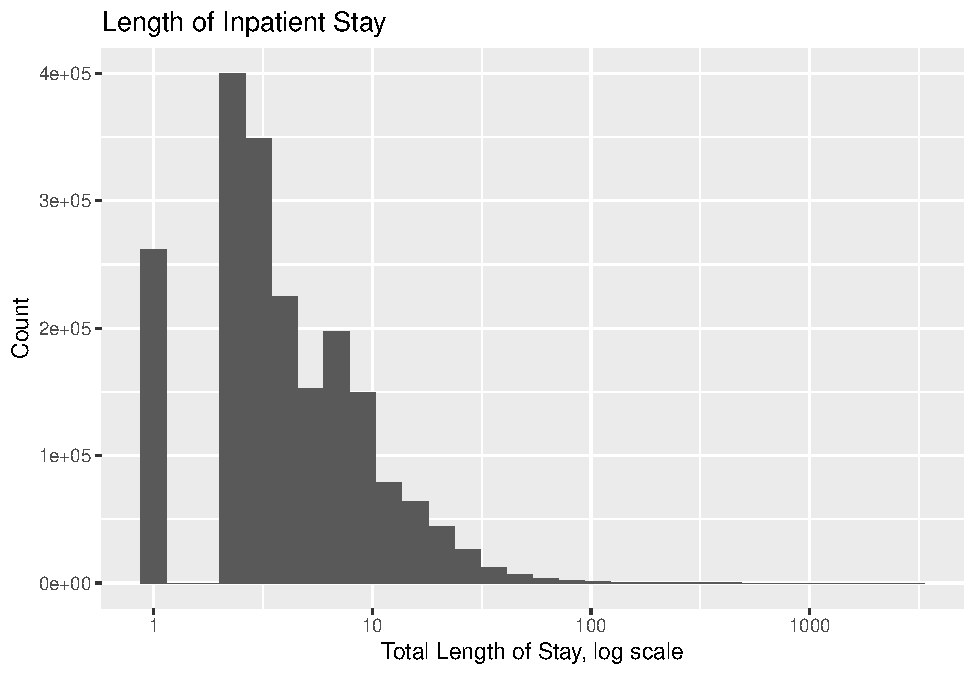
\includegraphics{final-project-paper_files/figure-latex/los-1.pdf}

\begin{Shaded}
\begin{Highlighting}[]
\KeywordTok{summary}\NormalTok{(ade\_flag}\OperatorTok{$}\NormalTok{LOS\_X)  }
\end{Highlighting}
\end{Shaded}

\begin{verbatim}
##     Min.  1st Qu.   Median     Mean  3rd Qu.     Max. 
##    0.000    2.000    3.000    5.651    6.000 2923.000
\end{verbatim}

\begin{Shaded}
\begin{Highlighting}[]
\NormalTok{ade\_flag }\OperatorTok{\%\textgreater{}\%}
\StringTok{  }\KeywordTok{ggplot}\NormalTok{(}\KeywordTok{aes}\NormalTok{(}\DataTypeTok{x =}\NormalTok{ LOS\_X, }\DataTypeTok{fill =}\NormalTok{ DIED }\OperatorTok{==}\StringTok{ }\DecValTok{0}\NormalTok{)) }\OperatorTok{+}
\StringTok{  }\KeywordTok{geom\_histogram}\NormalTok{() }\OperatorTok{+}
\StringTok{  }\KeywordTok{scale\_x\_continuous}\NormalTok{(}\DataTypeTok{trans =} \StringTok{\textquotesingle{}log10\textquotesingle{}}\NormalTok{)}
\end{Highlighting}
\end{Shaded}

\begin{verbatim}
## Warning: Transformation introduced infinite values in continuous x-axis
\end{verbatim}

\begin{verbatim}
## `stat_bin()` using `bins = 30`. Pick better value with `binwidth`.
\end{verbatim}

\begin{verbatim}
## Warning: Removed 43456 rows containing non-finite values (stat_bin).
\end{verbatim}

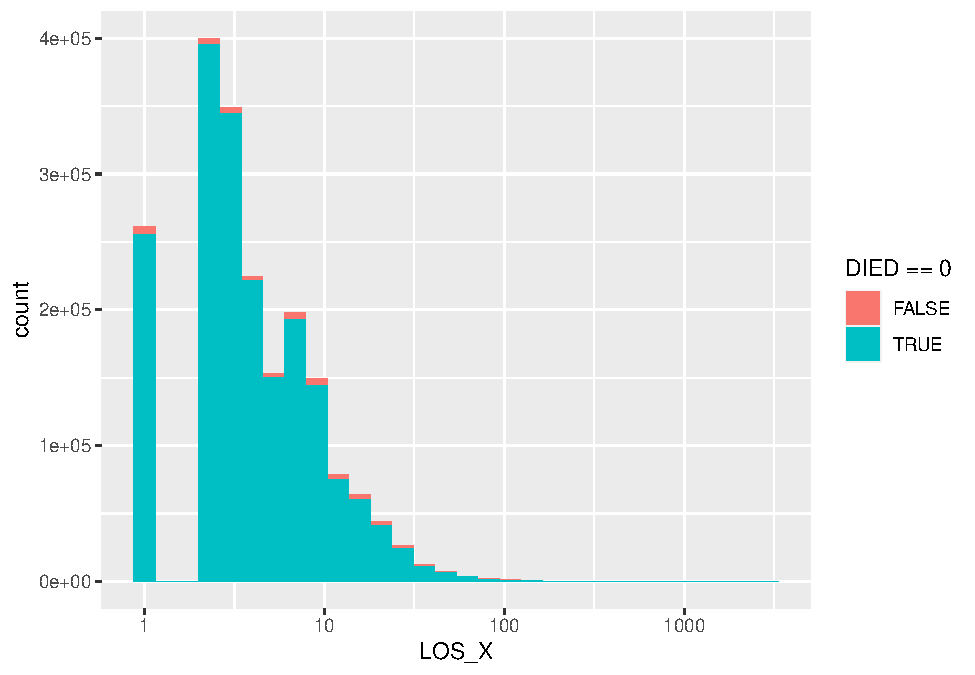
\includegraphics{final-project-paper_files/figure-latex/los-2.pdf}

\begin{Shaded}
\begin{Highlighting}[]
\NormalTok{ade\_flag }\OperatorTok{\%\textgreater{}\%}
\StringTok{  }\KeywordTok{filter}\NormalTok{(LOS\_X }\OperatorTok{\textless{}=}\StringTok{ }\DecValTok{10}\NormalTok{) }\OperatorTok{\%\textgreater{}\%}
\StringTok{  }\KeywordTok{ggplot}\NormalTok{(}\KeywordTok{aes}\NormalTok{(}\DataTypeTok{x =}\NormalTok{ LOS\_X, }\DataTypeTok{fill =}\NormalTok{ DIED }\OperatorTok{==}\StringTok{ }\DecValTok{0}\NormalTok{)) }\OperatorTok{+}
\StringTok{  }\KeywordTok{geom\_histogram}\NormalTok{() }\OperatorTok{+}
\StringTok{  }\KeywordTok{scale\_x\_discrete}\NormalTok{()}
\end{Highlighting}
\end{Shaded}

\begin{verbatim}
## `stat_bin()` using `bins = 30`. Pick better value with `binwidth`.
\end{verbatim}

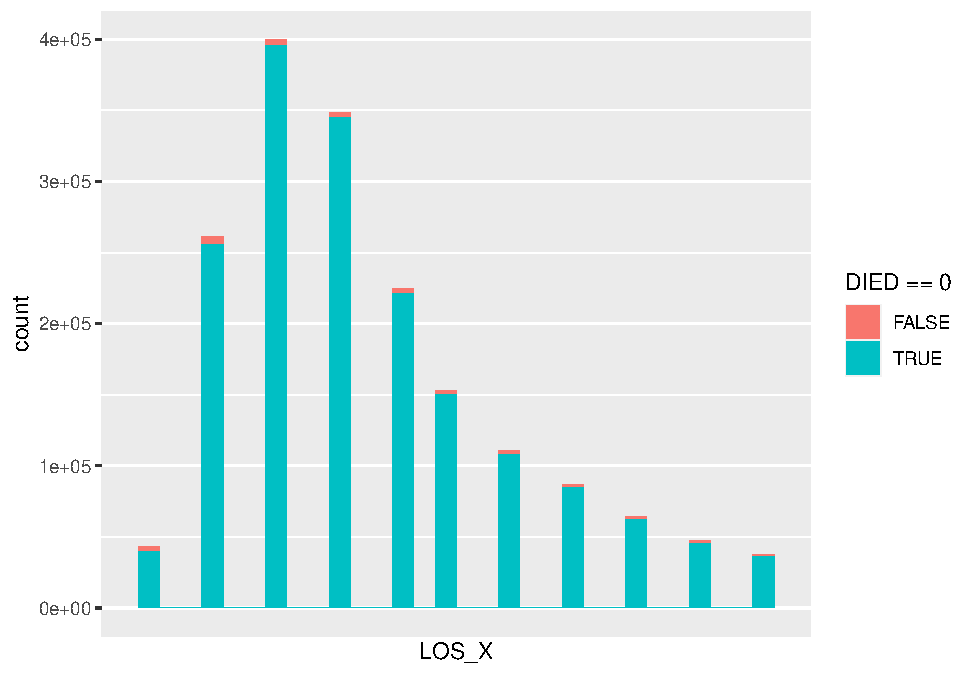
\includegraphics{final-project-paper_files/figure-latex/los-3.pdf}

\begin{Shaded}
\begin{Highlighting}[]
\KeywordTok{hist}\NormalTok{(ade\_flag}\OperatorTok{$}\NormalTok{LOS\_X[ade\_flag}\OperatorTok{$}\NormalTok{LOS\_X }\OperatorTok{\textless{}}\StringTok{ }\DecValTok{10}\NormalTok{])}
\end{Highlighting}
\end{Shaded}

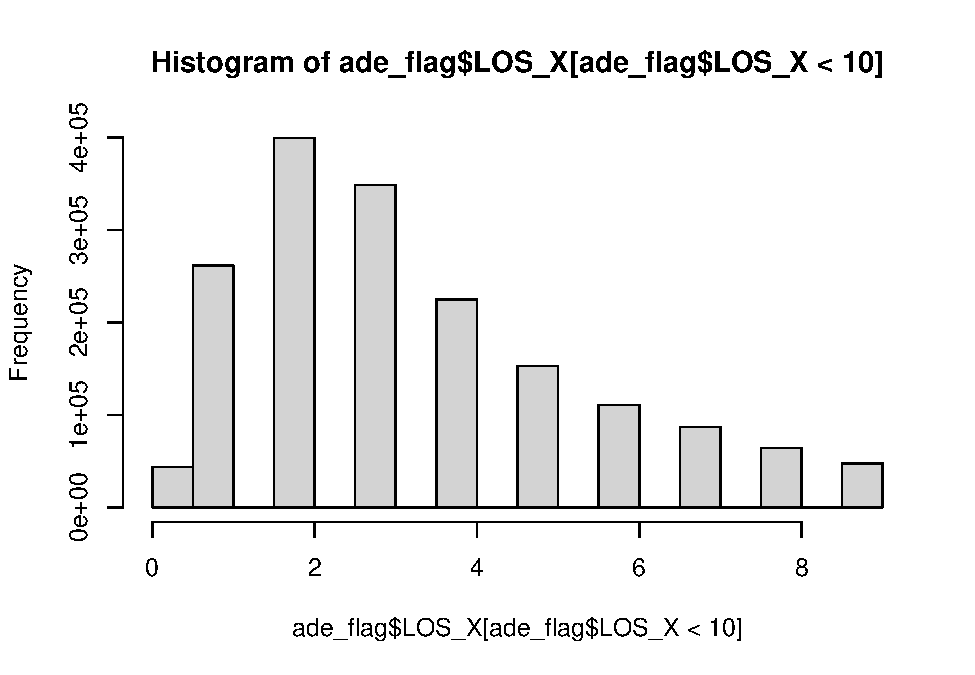
\includegraphics{final-project-paper_files/figure-latex/los-4.pdf}

\begin{Shaded}
\begin{Highlighting}[]
\CommentTok{\#\#{-}Proportion who died }

\NormalTok{ade\_flag }\OperatorTok{\%\textgreater{}\%}
\StringTok{    }\KeywordTok{summarize}\NormalTok{(}\DataTypeTok{PCT\_DIED =} \KeywordTok{mean}\NormalTok{(DIED, }\DataTypeTok{na.rm =} \OtherTok{TRUE}\NormalTok{))}
\end{Highlighting}
\end{Shaded}

\begin{verbatim}
## # A tibble: 1 x 1
##   PCT_DIED
##      <dbl>
## 1   0.0240
\end{verbatim}

\begin{Shaded}
\begin{Highlighting}[]
\NormalTok{ade\_flag }\OperatorTok{\%\textgreater{}\%}
\StringTok{  }\KeywordTok{summarize}\NormalTok{(}\DataTypeTok{sd\_died =} \KeywordTok{sd}\NormalTok{(DIED, }\DataTypeTok{na.rm =} \OtherTok{TRUE}\NormalTok{))}
\end{Highlighting}
\end{Shaded}

\begin{verbatim}
## # A tibble: 1 x 1
##   sd_died
##     <dbl>
## 1   0.153
\end{verbatim}

\begin{Shaded}
\begin{Highlighting}[]
\CommentTok{\#\#{-}Average cost per day }
\NormalTok{ade\_cost \textless{}{-}}\StringTok{ }\NormalTok{ade\_flag }
\NormalTok{ade\_cost}\OperatorTok{$}\NormalTok{LOS\_X[ade\_cost}\OperatorTok{$}\NormalTok{LOS\_X }\OperatorTok{==}\StringTok{ }\DecValTok{0}\NormalTok{] \textless{}{-}}\StringTok{ }\DecValTok{1}
\NormalTok{ade\_cost \textless{}{-}}\StringTok{ }\NormalTok{ade\_cost }\OperatorTok{\%\textgreater{}\%}
\StringTok{  }\KeywordTok{filter}\NormalTok{(}\OperatorTok{!}\KeywordTok{is.na}\NormalTok{(LOS\_X), }\OperatorTok{!}\KeywordTok{is.na}\NormalTok{(TOTCHG\_X)) }\OperatorTok{\%\textgreater{}\%}
\StringTok{        }\KeywordTok{mutate}\NormalTok{(}\DataTypeTok{cost\_per\_day =} \KeywordTok{round}\NormalTok{(TOTCHG\_X}\OperatorTok{/}\NormalTok{LOS\_X, }\DecValTok{2}\NormalTok{))}
\NormalTok{ade\_cost }\OperatorTok{\%\textgreater{}\%}
\StringTok{    }\KeywordTok{summarize}\NormalTok{(}\DataTypeTok{avg\_cost\_per\_day =} \KeywordTok{round}\NormalTok{(}\KeywordTok{mean}\NormalTok{(cost\_per\_day, }\DataTypeTok{na.rm =} \OtherTok{TRUE}\NormalTok{),}\DecValTok{2}\NormalTok{))}
\end{Highlighting}
\end{Shaded}

\begin{verbatim}
## # A tibble: 1 x 1
##   avg_cost_per_day
##              <dbl>
## 1           13395.
\end{verbatim}

\begin{Shaded}
\begin{Highlighting}[]
\NormalTok{ade\_cost }\OperatorTok{\%\textgreater{}\%}
\StringTok{        }\KeywordTok{mutate}\NormalTok{(}\DataTypeTok{cost\_per\_day =} \KeywordTok{round}\NormalTok{(TOTCHG\_X}\OperatorTok{/}\NormalTok{LOS\_X, }\DecValTok{2}\NormalTok{)) }\OperatorTok{\%\textgreater{}\%}\StringTok{ }
\StringTok{        }\KeywordTok{summarize}\NormalTok{(}\DataTypeTok{sd\_daily\_cost =} \KeywordTok{sd}\NormalTok{(cost\_per\_day, }\DataTypeTok{na.rm =} \OtherTok{TRUE}\NormalTok{))}
\end{Highlighting}
\end{Shaded}

\begin{verbatim}
## # A tibble: 1 x 1
##   sd_daily_cost
##           <dbl>
## 1        17466.
\end{verbatim}

\begin{Shaded}
\begin{Highlighting}[]
\NormalTok{ade\_cost }\OperatorTok{\%\textgreater{}\%}
\StringTok{  }\KeywordTok{ggplot}\NormalTok{(}\KeywordTok{aes}\NormalTok{(}\DataTypeTok{x =}\NormalTok{ cost\_per\_day)) }\OperatorTok{+}
\StringTok{  }\KeywordTok{geom\_histogram}\NormalTok{() }\OperatorTok{+}
\StringTok{  }\KeywordTok{scale\_x\_continuous}\NormalTok{(}\DataTypeTok{trans =} \StringTok{\textquotesingle{}log10\textquotesingle{}}\NormalTok{, }\DataTypeTok{labels =}\NormalTok{ scales}\OperatorTok{::}\StringTok{ }\KeywordTok{dollar\_format}\NormalTok{()) }\OperatorTok{+}
\StringTok{  }\KeywordTok{labs}\NormalTok{(}\DataTypeTok{x =} \StringTok{\textquotesingle{}Average cost per day of Hospital Admission, USD\textquotesingle{}}\NormalTok{, }\DataTypeTok{y =} \StringTok{\textquotesingle{}Count\textquotesingle{}}\NormalTok{, }\DataTypeTok{title =} \StringTok{\textquotesingle{}Average Cost Per day of Inpatient Visit\textquotesingle{}}\NormalTok{)}
\end{Highlighting}
\end{Shaded}

\begin{verbatim}
## `stat_bin()` using `bins = 30`. Pick better value with `binwidth`.
\end{verbatim}

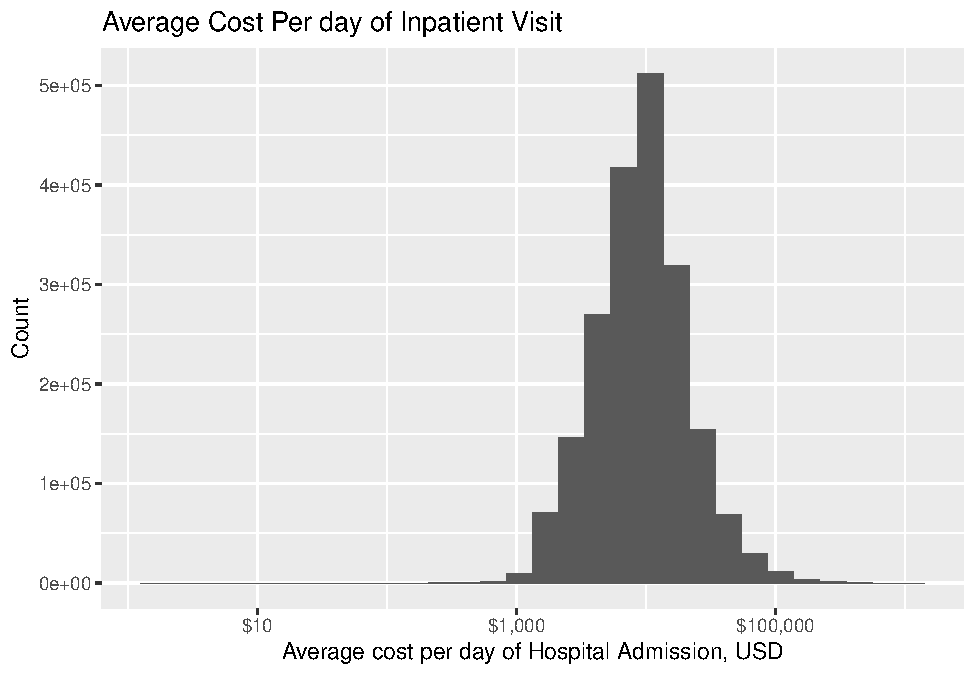
\includegraphics{final-project-paper_files/figure-latex/cost-per-day-1.pdf}

\#\#-Most common procedures \#\#-Map of NY \#\#-Breakdown of Patients by
Region \#\#-Bivariate choropleth map of admissions versus ade's

\begin{Shaded}
\begin{Highlighting}[]
\NormalTok{nycounties \textless{}{-}}\StringTok{ }\NormalTok{rgdal}\OperatorTok{::}\KeywordTok{readOGR}\NormalTok{(}\StringTok{\textquotesingle{}https://raw.githubusercontent.com/hillt5/DATA608/main/Final\%20Project/gz\_2010\_us\_050\_00\_20m.json\textquotesingle{}}\NormalTok{)}
\end{Highlighting}
\end{Shaded}

\begin{verbatim}
## OGR data source with driver: GeoJSON 
## Source: "https://raw.githubusercontent.com/hillt5/DATA608/main/Final%20Project/gz_2010_us_050_00_20m.json", layer: "gz_2010_us_050_00_20m"
## with 3221 features
## It has 6 fields
\end{verbatim}

\begin{Shaded}
\begin{Highlighting}[]
\NormalTok{nycounties \textless{}{-}}\StringTok{ }\NormalTok{nycounties[nycounties}\OperatorTok{$}\NormalTok{STATE }\OperatorTok{==}\StringTok{ }\DecValTok{36}\NormalTok{,]}
\end{Highlighting}
\end{Shaded}

\#\#Most common admitting diagnosis

\begin{Shaded}
\begin{Highlighting}[]
\NormalTok{ade\_flag }\OperatorTok{\%\textgreater{}\%}\StringTok{ }\CommentTok{\#most common ADEs}
\StringTok{  }\KeywordTok{group\_by}\NormalTok{(Code) }\OperatorTok{\%\textgreater{}\%}
\StringTok{  }\KeywordTok{summarize}\NormalTok{(}\DataTypeTok{n\_pt =} \KeywordTok{n}\NormalTok{()) }\OperatorTok{\%\textgreater{}\%}
\StringTok{  }\KeywordTok{arrange}\NormalTok{(}\KeywordTok{desc}\NormalTok{(n\_pt))}
\end{Highlighting}
\end{Shaded}

\begin{verbatim}
## # A tibble: 72 x 2
##    Code     n_pt
##    <chr>   <int>
##  1 <NA>  1973695
##  2 D6959   17374
##  3 I952     5047
##  4 K521     4075
##  5 L270     3655
##  6 N141     2811
##  7 G620     2262
##  8 L271      960
##  9 R502      752
## 10 N990      698
## # ... with 62 more rows
\end{verbatim}

\begin{Shaded}
\begin{Highlighting}[]
\NormalTok{ade\_admitting \textless{}{-}}\StringTok{ }\NormalTok{ade\_flag }\OperatorTok{\%\textgreater{}\%}\StringTok{ }\CommentTok{\#most common ADEs, admitting only}
\StringTok{  }\NormalTok{dplyr}\OperatorTok{::}\KeywordTok{select}\NormalTok{(I10\_DX\_Admitting) }\OperatorTok{\%\textgreater{}\%}
\StringTok{  }\KeywordTok{group\_by}\NormalTok{(I10\_DX\_Admitting) }\OperatorTok{\%\textgreater{}\%}
\StringTok{  }\KeywordTok{summarize}\NormalTok{(}\DataTypeTok{n\_patients =} \KeywordTok{n}\NormalTok{()) }\OperatorTok{\%\textgreater{}\%}
\StringTok{  }\KeywordTok{arrange}\NormalTok{(}\KeywordTok{desc}\NormalTok{(n\_patients)) }\OperatorTok{\%\textgreater{}\%}
\StringTok{  }\KeywordTok{head}\NormalTok{(}\DecValTok{10}\NormalTok{) }\OperatorTok{\%\textgreater{}\%}
\StringTok{  }\KeywordTok{left\_join}\NormalTok{(icd, }\KeywordTok{c}\NormalTok{(}\StringTok{\textquotesingle{}I10\_DX\_Admitting\textquotesingle{}}\NormalTok{ =}\StringTok{ \textquotesingle{}V3\textquotesingle{}}\NormalTok{)) }\OperatorTok{\%\textgreater{}\%}
\StringTok{  }\KeywordTok{select}\NormalTok{(V5, n\_patients)}

\KeywordTok{ggplot}\NormalTok{(ade\_admitting, }\KeywordTok{aes}\NormalTok{(}\DataTypeTok{x =} \KeywordTok{fct\_reorder}\NormalTok{(V5, n\_patients), }\DataTypeTok{y =}\NormalTok{ n\_patients)) }\OperatorTok{+}
\StringTok{  }\KeywordTok{geom\_col}\NormalTok{() }\OperatorTok{+}
\StringTok{  }\KeywordTok{coord\_flip}\NormalTok{()}
\end{Highlighting}
\end{Shaded}

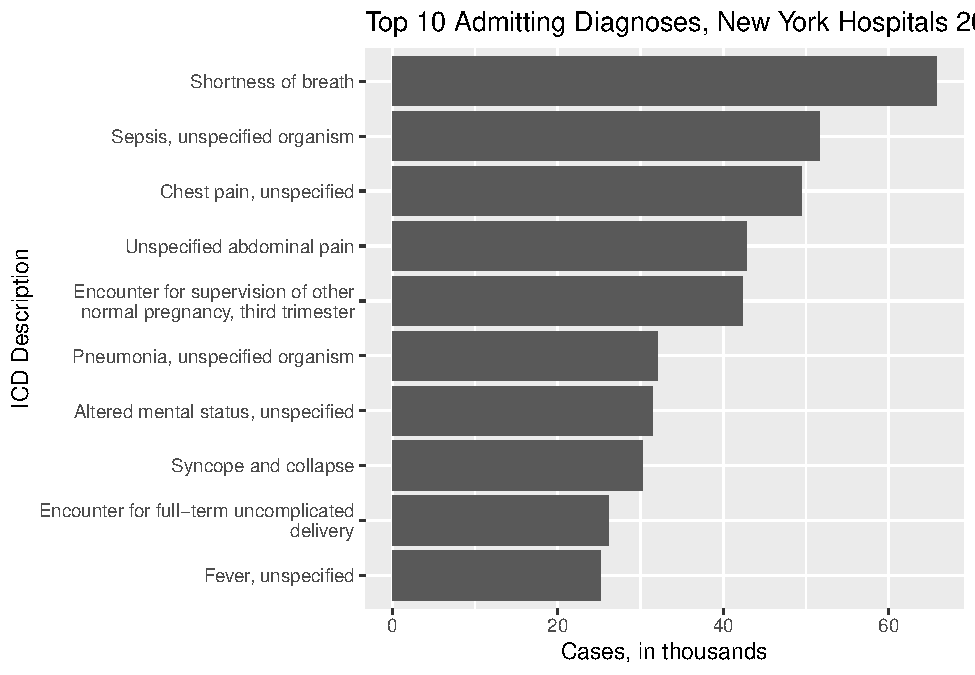
\includegraphics{final-project-paper_files/figure-latex/dx-admitting-1.pdf}
\#\#-Most common procedures

\begin{Shaded}
\begin{Highlighting}[]
\KeywordTok{ggplot}\NormalTok{(ade\_flag, }\KeywordTok{aes}\NormalTok{(I10\_NPR)) }\OperatorTok{+}\StringTok{ }\CommentTok{\#anomaly in the number of procedures}
\StringTok{  }\KeywordTok{geom\_bar}\NormalTok{()}
\end{Highlighting}
\end{Shaded}

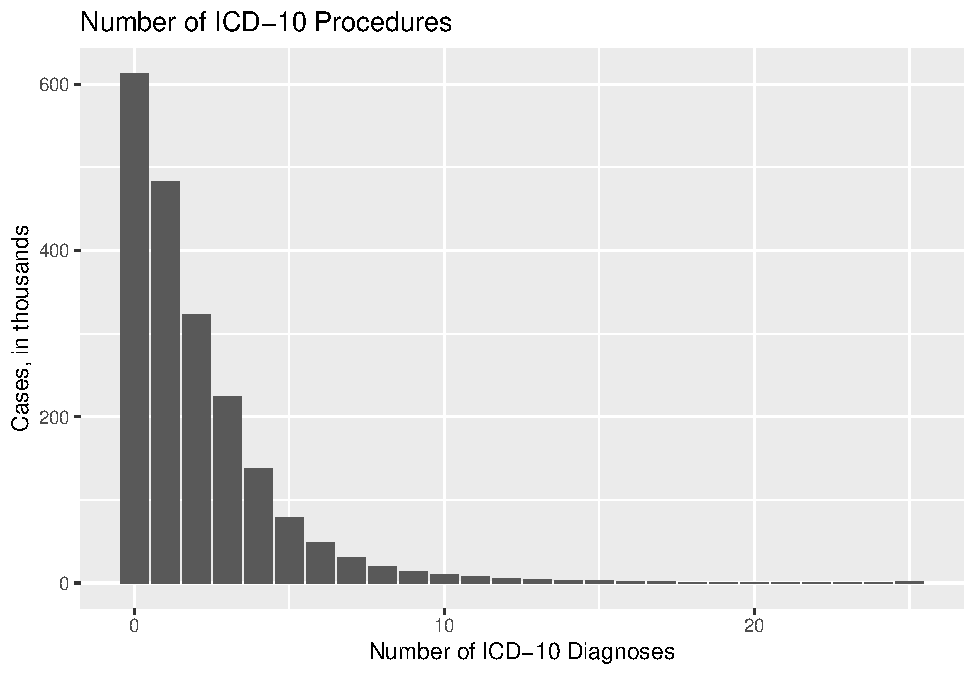
\includegraphics{final-project-paper_files/figure-latex/n-procedures-1.pdf}

\begin{Shaded}
\begin{Highlighting}[]
\NormalTok{i10\_procedure \textless{}{-}}\StringTok{ }\KeywordTok{read.csv}\NormalTok{(}\StringTok{\textquotesingle{}i10\_procedure.csv\textquotesingle{}}\NormalTok{)}


\NormalTok{proc\_counts \textless{}{-}}\StringTok{ }\NormalTok{ade\_flag }\OperatorTok{\%\textgreater{}\%}\StringTok{ }\CommentTok{\#use similar code to determine most common procedures}
\StringTok{  }\NormalTok{dplyr}\OperatorTok{::}\StringTok{ }\KeywordTok{select}\NormalTok{(I10\_PR1}\OperatorTok{:}\NormalTok{I10\_PR25) }\OperatorTok{\%\textgreater{}\%}
\StringTok{  }\KeywordTok{gather}\NormalTok{(dx\_num, Code, I10\_PR1}\OperatorTok{:}\NormalTok{I10\_PR25,}\DataTypeTok{factor\_key =} \OtherTok{TRUE}\NormalTok{ ) }\OperatorTok{\%\textgreater{}\%}
\StringTok{  }\KeywordTok{mutate}\NormalTok{(}\DataTypeTok{Code =} \KeywordTok{as.factor}\NormalTok{(Code)) }\OperatorTok{\%\textgreater{}\%}
\StringTok{  }\KeywordTok{group\_by}\NormalTok{(Code) }\OperatorTok{\%\textgreater{}\%}
\StringTok{  }\KeywordTok{summarize}\NormalTok{(}\DataTypeTok{n\_patients =} \KeywordTok{n}\NormalTok{()) }\OperatorTok{\%\textgreater{}\%}
\StringTok{  }\KeywordTok{mutate}\NormalTok{(}\DataTypeTok{Code =} \KeywordTok{na\_if}\NormalTok{(Code, }\StringTok{\textquotesingle{} \textquotesingle{}}\NormalTok{)) }\OperatorTok{\%\textgreater{}\%}
\StringTok{  }\KeywordTok{drop\_na}\NormalTok{() }\OperatorTok{\%\textgreater{}\%}
\StringTok{  }\KeywordTok{arrange}\NormalTok{(}\KeywordTok{desc}\NormalTok{(n\_patients)) }\OperatorTok{\%\textgreater{}\%}
\StringTok{  }\KeywordTok{inner\_join}\NormalTok{(i10\_procedure, }\DataTypeTok{by =} \KeywordTok{c}\NormalTok{(}\StringTok{\textquotesingle{}Code\textquotesingle{}}\NormalTok{ =}\StringTok{ \textquotesingle{}ICD.10.PCS.CODE\textquotesingle{}}\NormalTok{))  }\OperatorTok{\%\textgreater{}\%}\StringTok{ }\CommentTok{\#join with i10 procedure text csv}
\StringTok{  }\NormalTok{dplyr }\OperatorTok{::}\StringTok{ }\KeywordTok{select}\NormalTok{(ICD.}\FloatTok{10.}\NormalTok{PCS.CODE.DESCRIPTION, n\_patients, Code)}


\NormalTok{proc\_counts }\OperatorTok{\%\textgreater{}\%}
\StringTok{  }\KeywordTok{arrange}\NormalTok{(}\KeywordTok{desc}\NormalTok{(n\_patients)) }\OperatorTok{\%\textgreater{}\%}
\StringTok{  }\KeywordTok{head}\NormalTok{(}\DecValTok{10}\NormalTok{) }\OperatorTok{\%\textgreater{}\%}
\StringTok{  }\KeywordTok{ggplot}\NormalTok{(}\KeywordTok{aes}\NormalTok{(}\DataTypeTok{x =} \KeywordTok{fct\_reorder}\NormalTok{(ICD.}\FloatTok{10.}\NormalTok{PCS.CODE.DESCRIPTION, n\_patients))) }\OperatorTok{+}
\StringTok{  }\KeywordTok{geom\_col}\NormalTok{(}\KeywordTok{aes}\NormalTok{(}\DataTypeTok{y =}\NormalTok{ n\_patients}\OperatorTok{/}\DecValTok{1000}\NormalTok{)) }\OperatorTok{+}\StringTok{ }
\StringTok{  }\KeywordTok{scale\_x\_discrete}\NormalTok{(}\DataTypeTok{name =} \StringTok{\textquotesingle{}ICD Description\textquotesingle{}}\NormalTok{, }\DataTypeTok{labels =} \ControlFlowTok{function}\NormalTok{(x) }\KeywordTok{str\_wrap}\NormalTok{(}\KeywordTok{str\_replace\_all}\NormalTok{(x, }\StringTok{"foo"}\NormalTok{ , }\StringTok{" "}\NormalTok{), }\DataTypeTok{width =} \DecValTok{55}\NormalTok{)) }\OperatorTok{+}
\StringTok{  }\KeywordTok{theme}\NormalTok{(}\DataTypeTok{legend.position =} \KeywordTok{c}\NormalTok{(}\FloatTok{0.75}\NormalTok{,}\FloatTok{0.25}\NormalTok{)) }\OperatorTok{+}
\StringTok{  }\KeywordTok{labs}\NormalTok{(}\DataTypeTok{title =} \StringTok{\textquotesingle{}Top 10 Most Common Procedures, 2018\textquotesingle{}}\NormalTok{) }\OperatorTok{+}
\StringTok{  }\KeywordTok{scale\_y\_continuous}\NormalTok{(}\DataTypeTok{name =} \StringTok{\textquotesingle{}Procedure ClLaims, in thousands\textquotesingle{}}\NormalTok{) }\OperatorTok{+}
\StringTok{  }\KeywordTok{coord\_flip}\NormalTok{() }
\end{Highlighting}
\end{Shaded}

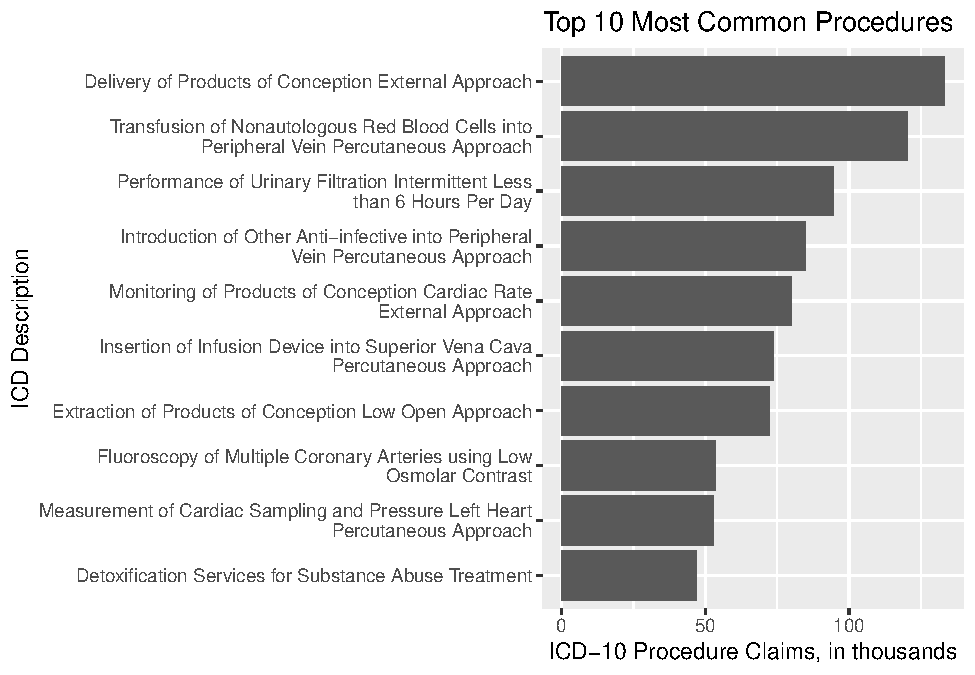
\includegraphics{final-project-paper_files/figure-latex/top-10-procedures-1.pdf}

\bibliography{mybibfile.bib}


\end{document}
